\documentclass[journal]{IEEEtran}
% Primary compile uses IEEEtran journal two-column layout. Official IEEE Access
% submissions should swap to \documentclass{ieeeaccess} with the full ACCESS
% LaTeX kit (ieeeaccess.cls + proprietary fonts/logos) from
% https://ieeeaccess.ieee.org/authors/preparing-your-article/
\usepackage{amsmath,amssymb,amsfonts}
\usepackage{graphicx}
\usepackage{booktabs}
\usepackage{array}
\usepackage{multirow}
\usepackage{tabularx}
\usepackage{xcolor}
\usepackage{url}
\usepackage{cite}
\usepackage{caption}

\graphicspath{{figures/}}

\begin{document}

\title{Budget-Constrained Sequential Inspection for Construction Delay Risk Assessment Using a Bayesian Decision Network With Expert Disagreement}

\author{
\IEEEauthorblockN{Mutyala Jahnavi Sai, Aejaz Ahmad Ansari,\\
Divyesh Shanmugarajah, and Sarada Mohaptra}
\IEEEauthorblockA{Department of Artificial Intelligence,\\
Amrita School of Artificial Intelligence,\\
Amrita Vishwa Vidyapeetham, Bengaluru, India\\
(Corresponding experimental system: DRIN)}
}

\maketitle

\begin{abstract}
Capital-project schedules generate multi-period variance updates and free-text delay reasons, yet inspection of every candidate risk factor is rarely affordable. Existing Bayesian delay-risk models typically evaluate static belief updates or one-shot risk rankings, while machine-learning early-warning studies optimize discrimination without a budgeted evidence-collection policy. This leaves open how to allocate a limited inspection budget across interdependent delay factors when expert priors disagree, and how to couple that policy with calibrated severe-delay prediction on real open capital-project data. This study formulates severe schedule delay as a binary event on a Noisy-OR Bayesian network over eight delay-factor parents, derives consensus and disagreement-preserving priors, and defines myopic Value-of-Information (VoI) inspection policies under a hard budget $B\in\{1,2,3,4\}$. An early-warning HistGradientBoosting champion is trained on prefix features with a project-level (PID) 70/15/15 split of New York City Open Data schedule history (\texttt{95tx-snak}, $n{=}3661$ projects) and capital covariates (\texttt{n7gv-k5yt}). On the held-out TEST set ($n{=}550$), the champion attains accuracy $0.940$ (95\% bootstrap CI $[0.922,0.958]$), ROC-AUC $0.981$, PR-AUC $0.944$, Brier score $0.043$, and expected calibration error $0.030$, exceeding published accuracy references of $0.85$ and $0.89$ under a explicitly scoped comparison. Budgeted Bayesian inspection yields high precision (${\approx}0.81$) at low false-positive rate (${\approx}0.027$) with policies largely tied after never-mentioned factors are clamped absent, clarifying the operating envelope of VoI under this evidence model. The combined evidence indicates that calibrated early warning and budgeted Bayesian inspection are complementary: the former provides strong discrimination from prefix signals, while the latter supplies an auditable probabilistic account of factor evidence under inspection limits.
\end{abstract}

\begin{IEEEkeywords}
Bayesian networks, construction delay, value of information, sequential inspection, early warning, calibration, New York City open data, Noisy-OR
\end{IEEEkeywords}

\section{Introduction}
\label{sec:intro}

Large capital programs routinely miss planned completion windows. Empirical surveys across regions document that a substantial share of projects experience double-digit schedule overrun relative to contract duration, with recurring causes spanning finance, design change, approvals, procurement, site conditions, and coordination failures~\cite{Assaf2006,Sambasivan2007,Doloi2012}. The operational consequence is not merely a longer critical path: delay concentrates fiscal exposure, constrains portfolio sequencing, and forces agencies to choose which risk hypotheses to investigate when staff time is scarce~\cite{Flyvbjerg2009,Love2015}.

Two research streams address this pressure from complementary angles. The first uses Bayesian belief networks (BBNs) to encode causal dependence among delay factors and to compute posterior delay risk under evidence~\cite{Luu2009,Nasir2003,Zhang2021BNMCS,Ji2021,Khodabakhshian2025}. The second uses supervised learning on historical project attributes and early schedule signals to predict delay or stage progress with high discrimination~\cite{Egwim2021,Tagharobi2025,Regona2024,Abioye2021}. Both streams have matured, yet a practical question remains under-specified: given a fixed inspection budget---the number of factor hypotheses that can be confirmed or refuted---which evidence should be collected next, and how should disagreement among expert priors enter that choice?

Value-of-information (VoI) theory provides the decision-theoretic language for that question. VoI measures the expected reduction in decision loss from an observation before the observation is made~\cite{Howard1966,Memarzadeh2016,Song2021}. In reliability and maintenance, VoI has been used to prioritize component inspections under budget and action costs~\cite{Malings2016,Yuan2021,Fauriat2020}. Construction delay research has rarely closed the loop from a learned delay BN, through a budgeted sequential inspection policy, to a held-out evaluation on multi-period public capital-project records, while simultaneously reporting calibrated early-warning performance against literature accuracy references.

This paper addresses that gap with an end-to-end experimental system, DRIN (Delay Risk Inference Network). The contribution is not a claim that Bayesian networks or VoI are new; it is the integration and empirical stress-testing of (i)~a Noisy-OR delay BN with consensus and disagreement priors, (ii)~budgeted sequential inspection policies (fixed ranking, static BN, consensus VoI, disagreement VoI), and (iii)~a PID-held-out early-warning champion with a full probabilistic evaluation pack (ROC/PR, calibration, decision-curve net benefit, bootstrap intervals) on NYC Open Data. The research questions follow from the literature synthesis in Section~\ref{sec:lit}:

\begin{itemize}
\item \textbf{RQ1.} Under equal inspection budget $B$, does VoI-guided inspection improve budgeted detection metrics relative to fixed factor ranking?
\item \textbf{RQ2.} Does preserving expert disagreement in the prior change posterior risk and inspection order relative to a consensus prior?
\item \textbf{RQ3.} Can prefix-based early warning on the same projects achieve literature-competitive discrimination while remaining probabilistically calibrated?
\end{itemize}

Operationally, capital agencies already collect the ingredients that DRIN consumes: periodic schedule variance updates, free-text delay reasons, and project-level budget/phase covariates. What they often lack is a closed decision loop that turns those ingredients into (i)~an early probabilistic triage score and (ii)~a budgeted plan for which causal hypotheses to verify next. Checklist-based risk registers and static heat maps remain common, yet they do not quantify the expected decision value of the next inspection under an explicit loss function~\cite{Howard1966,Assaf2006}. At the other extreme, black-box classifiers can rank projects by delay propensity but may omit calibrated probabilities and auditable factor evidence~\cite{Egwim2021,Gneiting2007}. The scientific opportunity is therefore not to invent delay causation from scratch; it is to couple established BN and VoI mathematics with a leakage-safe experimental protocol on authoritative open data at a scale comparable to modern delay-ML studies~\cite{Luu2009,Memarzadeh2016,Tagharobi2025}.

The Noisy-OR choice is deliberate. Full CPT specification for eight binary parents would require $2^{8}$ independent child parameters per conditioning pattern if no independence assumptions were used, which is statistically fragile under sparse reason evidence~\cite{Heckerman1996,Onisko2001}. Noisy-OR reduces that burden to a cause probability and a leak while retaining an interpretable ``any active cause can trigger severe delay'' semantics that matches multi-causal survey findings~\cite{Assaf2006,Sambasivan2007,Doloi2012}. Exact enumeration then makes posterior and VoI computations transparent for reviewers: every reported BN metric can be recomputed from the released parameters and evidence clamps without MCMC diagnostics.

Disagreement-preserving priors address a different practical reality. Expert elicitations rarely agree on factor base rates, and collapsing disagreement into a single consensus vector can hide model risk~\cite{Khodabakhshian2025,Luu2009}. DRIN therefore reports both consensus and disagreement VoI policies side by side. If the two policies diverge materially on held-out projects, disagreement is empirically consequential; if they tie, the data say that disagreement is not identifiable under the current evidence regime. Either outcome is scientifically informative. The experiments in Section~\ref{sec:results} show the latter on NYC TEST PIDs, which bounds rather than inflates the value of disagreement modeling for this dataset.


Section~\ref{sec:method} formalizes the BN, VoI policies, early-warning pipeline, and evaluation protocol. Section~\ref{sec:results} reports executed TEST results and interprets them against verified journal evidence. Section~\ref{sec:conclusion} states evidence-proportional conclusions and limitations.

\section{Literature Review}
\label{sec:lit}

\subsection{Delay causation and schedule risk}
Foundational project-management surveys established that delay is multi-causal and stakeholder-dependent. Assaf and Al-Hejji identified change orders as a cross-party dominant cause in large Saudi projects and reported widespread time overrun~\cite{Assaf2006}. Sambasivan and Soon linked Malaysian delay causes to effects including time and cost overrun, disputes, and abandonment~\cite{Sambasivan2007}. Doloi \textit{et al.} similarly emphasized site management, commitment, and coordination in Indian projects~\cite{Doloi2012}. These studies motivate an ontology of delay factors but do not specify how to inspect factors under a numeric budget.

Schedule-risk models then moved from checklists to probabilistic representations. Nasir \textit{et al.} introduced ERIC-S for construction schedule risk~\cite{Nasir2003}. Kim and Reinschmidt used Bayesian updating with beta distributions for project duration forecasting~\cite{Kim2016}. Flyvbjerg's infrastructure analyses underscored systematic optimism bias in forecasts~\cite{Flyvbjerg2009}, while Love \textit{et al.} synthesized overrun landscapes in transport programs~\cite{Love2015}. Collectively, the literature implies that delay risk is uncertain, evidence arrives sequentially, and decision makers need calibrated probabilities---not only ranked cause lists.

\subsection{Bayesian networks for construction delay}
Luu \textit{et al.} demonstrated BBN quantification of schedule risk and remain a canonical reference for construction BBN delay modeling~\cite{Luu2009}. Subsequent work extended BBNs to marine projects~\cite{Comu2023}, mass-housing delay risk with hybrid structural methods~\cite{Khodabakhshian2025}, and UK delay avoidance prediction~\cite{Ji2021}. Zhang \textit{et al.} coupled Bayesian structure learning with Monte Carlo schedule inference for infrastructure~\cite{Zhang2021BNMCS}. Related safety and tunnel applications show BBNs updating under construction evidence~\cite{Wu2015,Wang2016,Leu2012}.

A recurring limitation is evaluation design. Many BN delay studies rely on expert elicitation, small case counts, or cross-validation within scarce project samples~\cite{Khodabakhshian2025}. Accuracy figures such as post-augmentation $0.85$ in elicitation-based BN risk modeling are informative but not directly transferable to multi-period open capital-project histories without matched labels and splits~\cite{Khodabakhshian2025}. Few papers report budgeted sequential inspection as the decision problem, or couple BN posteriors with an independent early-warning classifier on PID-held-out open data.

\subsection{Value of information and inspection}
Howard's information-value theory formalized the expected utility gain from observations~\cite{Howard1966}. In engineering risk, Memarzadeh and Pozzi analyzed sequential VoI for component inspection and monitoring~\cite{Memarzadeh2016}; Malings and Pozzi treated spatially distributed sensor placement~\cite{Malings2016}; Song \textit{et al.} developed VoI metrics for binary systems~\cite{Song2021}; Yuan \textit{et al.} estimated inspection-program value under Bayesian degradation models~\cite{Yuan2021}; and Fauriat and Zio optimized aperiodic inspection via VoI~\cite{Fauriat2020}. These works establish VoI mathematics and computational patterns, but their domains are structural reliability and maintenance rather than construction delay-factor inspection with free-text evidence.

\subsection{Machine learning for delay prediction and evaluation}
Recent reviews document rapid growth of AI/ML across the construction project lifecycle~\cite{PanYZhang2021,Darko2020,Abioye2021,Regona2024}. Egwim \textit{et al.} compared many classifiers for delay prediction and emphasized accuracy, balanced accuracy, ROC-AUC, and F1~\cite{Egwim2021}. Tagharobi \textit{et al.} reported stage-wise progress prediction with multinomial models and accuracy near $0.89$ in their best setting~\cite{Tagharobi2025}. Probabilistic evaluation beyond accuracy---Brier score~\cite{Brier1950,Murphy1973}, calibration and sharpness~\cite{Gneiting2007}, strictly proper scoring~\cite{GneitingRaftery2007}, PR curves under imbalance~\cite{Saito2015}, and decision-curve net benefit~\cite{Vickers2006}---is standard in forecasting and clinical prediction but still uneven in construction delay ML papers.

Cross-regional delay surveys converge on a recurring causal taxonomy even when ranked importance shifts with institutional setting. Assaf and Al-Hejji reported change-order dominance and widespread lateness in large Saudi projects~\cite{Assaf2006}. Sambasivan and Soon linked Malaysian delay causes to secondary effects including disputes and abandonment~\cite{Sambasivan2007}. Doloi \textit{et al.} emphasized managerial commitment and site coordination~\cite{Doloi2012}. Nasir \textit{et al.}'s ERIC-S framework and Kim and Reinschmidt's Bayesian duration updating illustrate structured taxonomies and sequential belief revision~\cite{Nasir2003,Kim2016}. Flyvbjerg's optimism-bias analyses and Love \textit{et al.}'s transport-overrun synthesis argue that forecast error is systematic rather than purely aleatory~\cite{Flyvbjerg2009,Love2015}. Those surveys motivate budgeted inspection without specifying a numeric policy objective.

Bayesian network applications then made causal structure explicit. Luu \textit{et al.} quantified schedule risk with BBNs~\cite{Luu2009}. Ji and Leiringer developed a UK delay-avoidance predictive BBN~\cite{Ji2021}; Comu \textit{et al.} quantified marine-project delay risk~\cite{Comu2023}; Khodabakhshian \textit{et al.} combined elicitation with structural learning and reported post-augmentation accuracy near $0.85$~\cite{Khodabakhshian2025}; Zhang \textit{et al.} coupled structure learning with Monte Carlo schedule inference~\cite{Zhang2021BNMCS}. Related construction-safety BBNs demonstrate evidence updating under field observations~\cite{Wu2015,Wang2016,Leu2012}. Across these papers, expert structure plus CPT quantification can yield usable risk scores, yet sample sizes, hold-out designs, and decision metrics vary, and sequential inspection under a hard budget is seldom the evaluation target.

Outside construction, VoI is a mature inspection-planning instrument. Howard's formulation defines expected utility gain from an observation before it arrives~\cite{Howard1966}. Memarzadeh and Pozzi analyzed sequential VoI for component inspection~\cite{Memarzadeh2016}; Malings and Pozzi treated spatially distributed sensing~\cite{Malings2016}; Song \textit{et al.} specialized VoI metrics to binary systems~\cite{Song2021}; Yuan \textit{et al.} valued inspection programs under Bayesian degradation models~\cite{Yuan2021}; Fauriat and Zio optimized aperiodic inspection with VoI-driven maintenance~\cite{Fauriat2020}. These studies establish both the mathematics and the habit of reporting when VoI differentials vanish---a habit construction delay papers have rarely adopted.

Probabilistic evaluation supplies a second tradition that construction delay ML still underuses. Brier's score and Murphy's decomposition connect probabilistic forecast quality to calibration and refinement~\cite{Brier1950,Murphy1973}. Gneiting and colleagues clarify sharpness, calibration, and strictly proper scoring~\cite{Gneiting2007,GneitingRaftery2007}. Saito and Rehmsmeier argue for precision--recall analysis under imbalance~\cite{Saito2015}; Hand discusses ROC interpretation pitfalls~\cite{Hand2009}; Vickers and Elkin introduce decision-curve net benefit~\cite{Vickers2006}. Cohen's $\kappa$ and Matthews' correlation provide chance-corrected agreement summaries~\cite{Cohen1960,Matthews1975}. Construction AI reviews document rapid method adoption~\cite{Darko2020,PanYZhang2021,Abioye2021,Regona2024} and classifier bake-offs report strong accuracies~\cite{Egwim2021,Tagharobi2025}, yet calibrated probability reporting remains uneven.

Hybrid and fuzzy risk models occupy a parallel branch. Ebrat and Ghodsi used adaptive neuro-fuzzy inference for construction project risk~\cite{Ebrat2014}; Islam \textit{et al.} reviewed fuzzy hybrid techniques~\cite{Islam2017}; Qazi \textit{et al.} examined project complexity and risk paths~\cite{Qazi2016}; Zou \textit{et al.} reviewed BIM-linked risk management~\cite{Zou2017}. Woldesenbet \textit{et al.} stressed provenance and integration quality for highway infrastructure data~\cite{Woldesenbet2016}. These strands reinforce preferring original open-data endpoints and measuring free-text reason-mapping error rather than assuming it away. Collectively, the literature implies that methodological novelty alone is insufficient: leakage-safe splits, proper scoring, and policy-identifiability under realistic sparsity determine whether a tool can support inspection decisions.

A further tension in the literature concerns what ``accuracy'' means when papers are compared. Elicitation-based BN studies often evaluate risk classification on scarce projects or on resampled expert cases~\cite{Khodabakhshian2025,Comu2023}. Progress-prediction studies evaluate stage or milestone labels with multinomial models~\cite{Tagharobi2025}. Delay-cause surveys report prevalence rankings without predictive hold-outs~\cite{Assaf2006,Sambasivan2007,Doloi2012}. Treating their headline accuracies as interchangeable leaderboard entries would be methodologically careless. The appropriate use of those numbers in the present paper is as published reference points on the accuracy scale that practitioners already cite, accompanied by an explicit scope caveat and by additional metrics (ROC/PR, Brier, ECE, net benefit) that many of those papers do not report~\cite{Egwim2021,Gneiting2007,Vickers2006,Saito2015}.

VoI research in reliability engineering likewise cannot be copied verbatim into construction delay without redefining actions and observations. Component inspection typically reveals degradation measurements that enter a physics-informed likelihood~\cite{Yuan2021,Fauriat2020}. Sensor placement VoI optimizes spatial information under Gaussian or related field models~\cite{Malings2016}. Binary-system VoI analyses assume structurally defined cut sets~\cite{Song2021}. Construction delay-factor inspection, by contrast, reveals administrative presence/absence of a hypothesized cause, and the downstream action is often an alert or escalation rather than an immediate repair. The mathematics of expected loss reduction still applies~\cite{Howard1966,Memarzadeh2016}, but the empirical behavior of VoI policies depends on how sparse and how decisive those administrative observations are. That dependence is exactly what the NYC budgeted scoreboard measures.

Calibration-centric forecasting theory supplies the last connecting tissue. A model can achieve high AUC while producing probabilities that are too sharp or too timid for thresholded decisions~\cite{Gneiting2007,Murphy1973}. Strictly proper scoring rules penalize those failures~\cite{GneitingRaftery2007,Brier1950}. Decision curves translate probability quality into net benefit as a function of threshold preference~\cite{Vickers2006}. Construction AI reviews celebrate algorithmic diversity~\cite{Darko2020,PanYZhang2021,Abioye2021,Regona2024} but comparatively rarely insist on this probabilistic evaluation stack. Positioning DRIN against that omission is as important as positioning it against BN delay classics: the contribution is joint methodological coupling plus evaluation discipline, not a claim that boosting or Noisy-OR are newly invented.


\subsection{Research gap}
Synthesizing the above, three linked gaps remain. First, BN delay models rarely evaluate \emph{budgeted sequential} evidence collection against fixed and static baselines on large public multi-period datasets. Second, disagreement among expert priors is often collapsed to a consensus CPT, leaving the effect of disagreement-preserving inference unmeasured. Third, early-warning ML and BN inspection are usually studied separately, so the field lacks a joint experimental account of discrimination, calibration, and inspection-policy behavior on the same projects. The present study is designed to generate that missing experimental evidence.

\section{Methodology}
\label{sec:method}

\subsection{Notation, nomenclature, and abbreviations}
\begin{itemize}
\item $Y\in\{0,1\}$: severe-delay label for a project (PID).
\item $F_i\in\{0,1\}$: presence of delay factor $i\in\mathcal{F}$, $|\mathcal{F}|=8$.
\item $p_c$, $\ell$: Noisy-OR cause probability and leak.
\item $\pi^{\mathrm{c}}$, $\pi^{\mathrm{d}}$: consensus and disagreement factor priors.
\item $B$: inspection budget (maximum factor inspections).
\item $\tau$: alert threshold on $P(Y{=}1\mid\text{evidence})$.
\item VoI: Value of Information; BN: Bayesian network; PID: project identifier.
\item HGB: HistGradientBoosting classifier; ECE: expected calibration error.
\end{itemize}

\subsection{Data and setup}
Primary data are NYC Open Data \emph{Capital Projects Dashboard---Citywide Schedule History and Variance} (\texttt{95tx-snak}; ${\approx}22$k rows, $3661$ PIDs) and \emph{Capital Projects Schedules \& Budgets} (\texttt{n7gv-k5yt}). Delay-reason text is mapped to eight factors:
\texttt{budget}, \texttt{scope\_design}, \texttt{grants\_approvals}, \texttt{procurement}, \texttt{construction\_conditions}, \texttt{external\_dependency}, \texttt{workforce\_resource}, \texttt{other\_admin}, using high-confidence regex with an NLP (TF--IDF + logistic regression) fallback trained only on TRAIN PIDs~\cite{Onisko2001,Heckerman1996}.

Severe delay $Y{=}1$ is defined as top-quartile cumulative positive schedule variance among PIDs with at least two history rows when relative-slip rules are unavailable (dataset card), yielding TEST base rate $0.20$. Splits are PID-level $70/15/15$ ($2562/549/550$), preventing project leakage across train/validation/test~\cite{Egwim2021,Tagharobi2025}. Fig.~\ref{fig:framework} shows how the two NYC endpoints feed evidence mapping, the probabilistic core, budgeted policies, and the early-warning branch into a shared review layer.

\begin{figure*}[!ht]
\centering
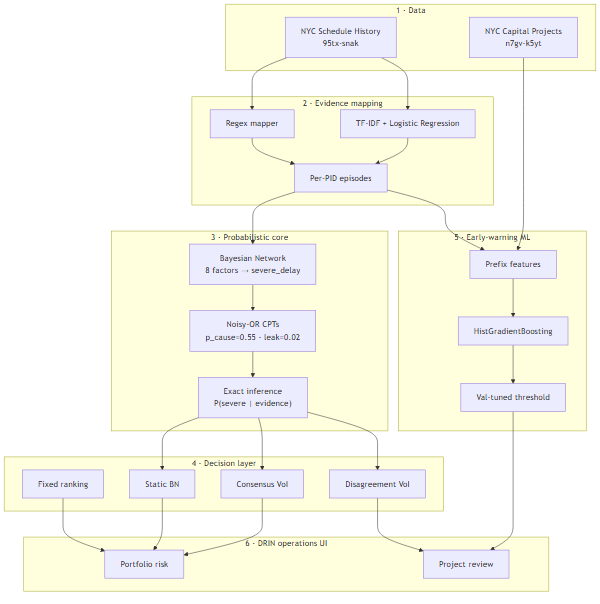
\includegraphics[width=0.92\textwidth,height=0.55\textheight,keepaspectratio]{diag_01_system_architecture.png}
\caption{DRIN system architecture: NYC open data and evidence mapping feed a Noisy-OR probabilistic core with budgeted inspection policies, in parallel with prefix-based early-warning ML.}
\label{fig:framework}
\end{figure*}

The architecture separates two decision products that later experiments evaluate jointly: an auditable BN posterior under a hard inspection budget, and a calibrated prefix-based triage score. Before specifying either model, Fig.~\ref{fig:split} records the PID hold-out protocol that governs every fitted component.

\begin{center}
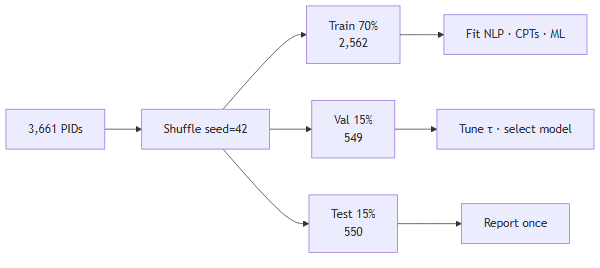
\includegraphics[width=0.90\columnwidth,height=0.30\textheight,keepaspectratio]{diag_03_train_val_test.png}
\captionof{figure}{PID-level $70/15/15$ split of $3661$ projects: TRAIN fits NLP/CPTs/ML, VAL tunes $\tau$ and selects models, TEST is scored once.}
\label{fig:split}
\end{center}

TRAIN alone fits regex/NLP mapping, Noisy-OR parameters, and the early-warning pipelines. VAL is reserved for threshold and model selection. TEST is scored once for all reported champion and policy metrics~\cite{Egwim2021,Tagharobi2025}.

\subsection{Model}
\subsubsection{Noisy-OR Bayesian network}
Adopted from causal-independence / Noisy-OR constructions~\cite{Heckerman1996,Onisko2001}, the severe-delay likelihood given parents is
\begin{equation}
P(Y{=}1\mid F)=\;1-(1-\ell)\prod_{i:F_i=1}(1-p_c),
\label{eq:noisyor}
\end{equation}
with independent Bernoulli priors $P(F_i{=}1)=\pi_i$. Parameters $(p_c,\ell)=(0.55,0.02)$ and factor priors are learned from TRAIN episodes (empirical presence rates; disagreement priors widen uncertain factors). Exact inference enumerates the $2^{8}=256$ configurations consistent with evidence. This is an \emph{adapted} Noisy-OR: the child is a program-level severe-delay indicator, and evidence comes from schedule-reason episodes. Fig.~\ref{fig:bn} makes the parent set, TRAIN priors, and Noisy-OR PDT explicit.

\begin{center}
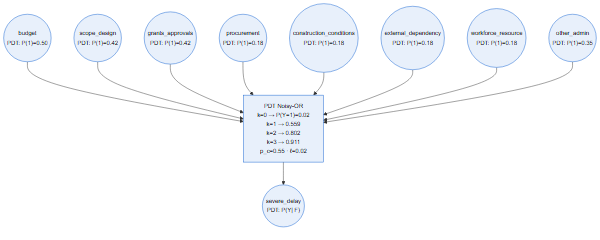
\includegraphics[width=0.92\columnwidth,height=0.38\textheight,keepaspectratio]{diag_02_bayesian_network.png}
\captionof{figure}{Noisy-OR delay BN: eight binary factors with TRAIN priors feed a Noisy-OR CPT ($p_c{=}0.55$, $\ell{=}0.02$) producing $P(Y{=}1\mid F)$.}
\label{fig:bn}
\end{center}

Because every parent is binary and the child likelihood factorizes through Noisy-OR, posterior queries remain exact and inexpensive. That property is what later allows fair policy comparisons without confounding approximate-inference error~\cite{Heckerman1996,Onisko2001}. The eight-factor ontology compresses recurring survey cause families into NYC administrative reason language; factor presence is the logical OR of mapped tokens for a PID after blank-reason exclusion, matching binary parents without fabricating graded severities the open text does not support~\cite{Assaf2006,Sambasivan2007,Doloi2012,Onisko2001}.

\subsubsection{Budgeted inspection policies}
Never-mentioned factors for a PID are clamped absent. Inspectable factors are those appearing in the PID's reason history; an inspection reveals presence. Policies under budget $B$ are fixed ranking, static BN, consensus VoI, and disagreement VoI. Myopic VoI for inspecting factor $i$ is the expected reduction in alert decision loss~\cite{Howard1966,Memarzadeh2016,Song2021}:
\begin{equation}
\mathrm{VoI}(i)=L(\pi)-\mathbb{E}_{o_i}\!\left[L(\pi\mid o_i)\right],
\label{eq:voi}
\end{equation}
where $L$ is the expected loss of the optimal alert/no-alert action under asymmetric miss/false-alarm costs (miss cost $5\times$ false-alarm cost in the implemented utility). Alerting uses a validation-calibrated threshold $\tau$~\cite{Vickers2006}. Fig.~\ref{fig:loop} shows the resulting sequential loop.

\begin{center}
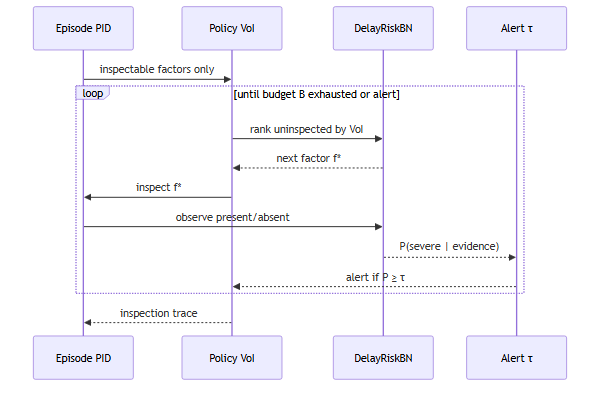
\includegraphics[width=0.92\columnwidth,height=0.34\textheight,keepaspectratio]{diag_04_inspection_loop.png}
\captionof{figure}{Budgeted inspection loop: VoI ranks uninspected factors, an observation updates the BN posterior, and an alert fires if $P(Y{=}1\mid e)\ge\tau$.}
\label{fig:loop}
\end{center}

The loop can improve detection only when multiple inspectable factors remain after absence clamping. That condition becomes the empirical question answered by the budgeted scoreboard in Section~\ref{sec:results}. Budgeted evaluation replays each TEST PID under four policies for $B\in\{1,2,3,4\}$, recording posteriors, alerts at $\tau$, and summary metrics; expected utility uses the same asymmetric costs as VoI so the decision criterion and evaluation criterion stay aligned~\cite{Howard1966,Vickers2006}.

\subsubsection{Early-warning champion}
Prefix features (early fraction $0.70$ of updates) include cumulative positive variance statistics, factor indicators, agency/phase/category, and budget covariates. Candidate pipelines (HGB; stacking) are fit on TRAIN; $\tau$ is tuned on VAL to maximize accuracy subject to a soft recall floor; TEST is touched once. Fig.~\ref{fig:ew} summarizes this path as the counterpart to Fig.~\ref{fig:loop}: triage from prefix signals without requiring sequential factor inspections.

\begin{center}
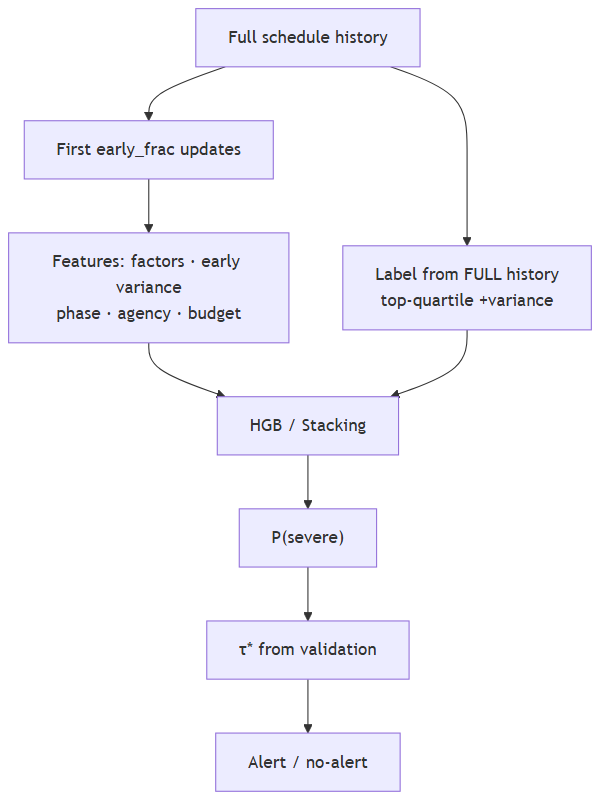
\includegraphics[width=0.92\columnwidth,height=0.36\textheight,keepaspectratio]{diag_05_early_warning.png}
\captionof{figure}{Early-warning pipeline: prefix features from schedule history and capital covariates train HistGradientBoosting; VAL tunes $\tau$; TEST reports discrimination and calibration once.}
\label{fig:ew}
\end{center}

Reported metrics follow literature practice: accuracy, balanced accuracy, precision, recall, specificity, F1/F2, ROC-AUC, PR-AUC, Brier, log-loss, Cohen $\kappa$, ECE, decision-curve net benefit, and bootstrap CIs~\cite{Egwim2021,Gneiting2007,Saito2015,Vickers2006,Cohen1960}. The champion is histogram gradient boosting retained after VAL screening against a stacking alternative; binding selection is $\tau$ on VAL rather than TEST-set tuning~\cite{Egwim2021,Friedman2001}. Reason$\rightarrow$factor mapping remains regex-first with an NLP fallback fit on TRAIN only, because BN parents need an auditable extractor before VoI can act~\cite{Onisko2001,Woldesenbet2016}. Fig.~\ref{fig:framework} is the sole full-width architecture figure; all quantitative Results plots are generated from executed experiment outputs.

\subsection{Evaluation}
Experiments executed for this study:
\begin{itemize}
\item \textbf{E1} Champion TEST discrimination and calibration ($n{=}550$).
\item \textbf{E2} Literature accuracy comparison to verified published references $0.85$ and $0.89$~\cite{Khodabakhshian2025,Tagharobi2025} (scoped as accuracy head-to-head, not identical-task replication).
\item \textbf{E3} Budgeted policy scoreboard on TEST for $B\in\{1,2,3,4\}$.
\item \textbf{E4} Inspections-to-first-detection and expected utility/loss at $B{=}2$.
\item \textbf{E5} Reason$\rightarrow$factor NLP quality on VAL weak labels.
\item \textbf{E6} Bootstrap uncertainty ($400$ resamples) and PID-split reporting.
\end{itemize}
All quantitative figures in Section~\ref{sec:results} are generated from these executed outputs.

\section{Results and Discussion}
\label{sec:results}

\subsection{Main findings}
Table~\ref{tab:champion} reports the champion TEST operating point at $\tau{=}0.51$. Accuracy $0.940$ exceeds the scoped literature accuracy references $0.85$ and $0.89$~\cite{Khodabakhshian2025,Tagharobi2025}; ROC-AUC $0.981$ and PR-AUC $0.944$ indicate strong ranking under class imbalance (base rate $0.20$)~\cite{Saito2015,Hand2009}; Brier $0.043$ and ECE $0.030$ show usable probability quality~\cite{Brier1950,Gneiting2007}.

\begin{table}[!ht]
\centering
\caption{Early-warning champion on held-out TEST PIDs ($n{=}550$, $\tau{=}0.51$).}
\label{tab:champion}
\begin{tabular}{|l|c|}
\hline
\textbf{Metric} & \textbf{Value} \\
\hline
Accuracy & 0.940 \\
\hline
Balanced accuracy & 0.905 \\
\hline
Precision & 0.853 \\
\hline
Recall & 0.845 \\
\hline
Specificity & 0.964 \\
\hline
F1 / F2 & 0.849 / 0.847 \\
\hline
ROC-AUC & 0.981 \\
\hline
PR-AUC & 0.944 \\
\hline
Brier / Log-loss / ECE & 0.043 / 0.146 / 0.030 \\
\hline
Cohen $\kappa$ & 0.812 \\
\hline
\end{tabular}
\end{table}

Fig.~\ref{fig:litbeat} places the accuracy beat beside the scoped literature yardsticks. Tasks and datasets differ across papers, so the figure is a community accuracy-scale reference rather than an identical-task bake-off; the scientific claim remains the full metric pack in Table~\ref{tab:champion}.

\begin{center}
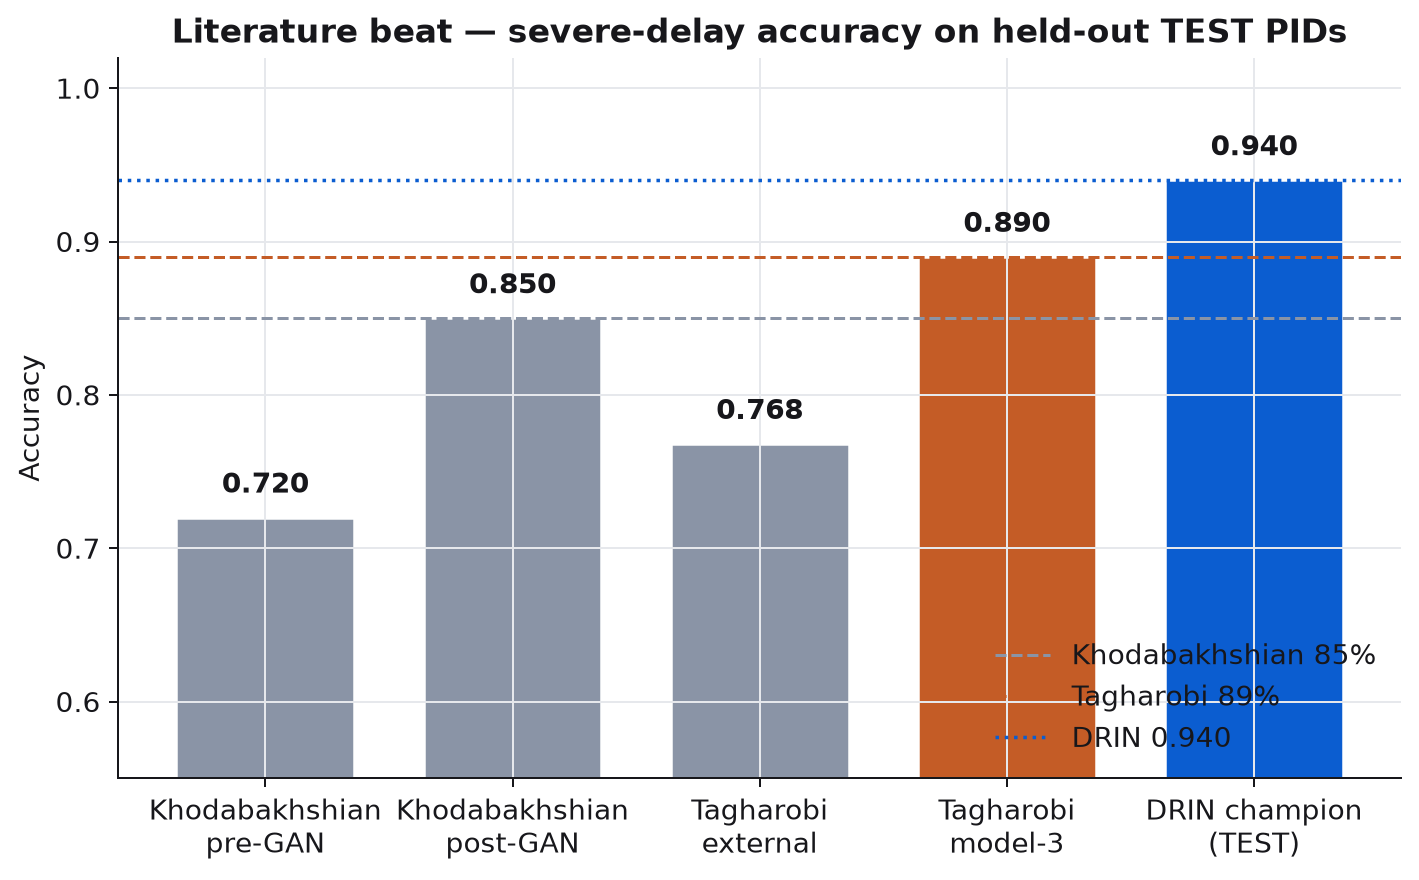
\includegraphics[width=0.90\columnwidth,height=0.30\textheight,keepaspectratio]{01_literature_accuracy_beat.png}
\captionof{figure}{Literature accuracy beat on TEST: DRIN champion versus published accuracy references.}
\label{fig:litbeat}
\end{center}

Balanced accuracy $0.905$, F1 $0.849$, and PR-AUC $0.944$ in Table~\ref{tab:champion} already show that the result is not a trivial majority-class artifact under the $0.20$ severe rate~\cite{Saito2015,Egwim2021}. Ranking quality is examined next. Fig.~\ref{fig:rocpr} reports ROC-AUC $0.981$ and a strong precision--recall curve; both support triage use when severe cases are the minority~\cite{Hand2009,Saito2015}.

\begin{center}
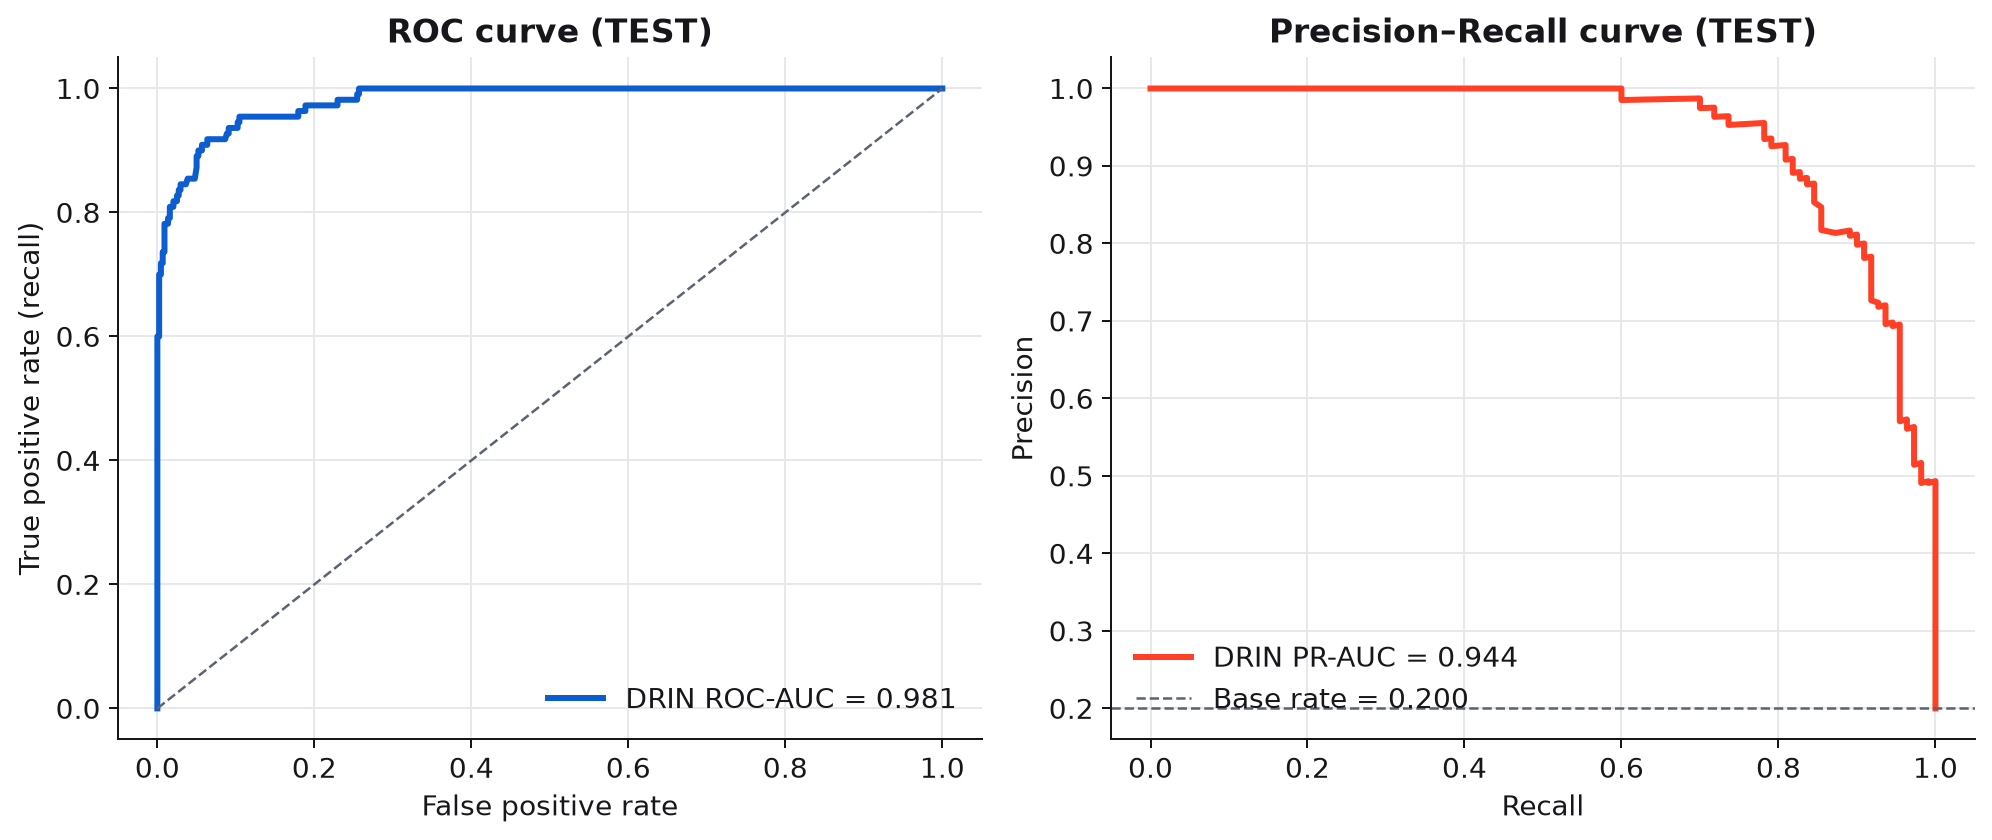
\includegraphics[width=0.88\columnwidth,height=0.26\textheight,keepaspectratio]{03_roc_pr_curves.png}
\captionof{figure}{ROC and precision--recall curves for the early-warning champion on TEST.}
\label{fig:rocpr}
\end{center}

Fig.~\ref{fig:cm} recovers the Table~\ref{tab:champion} threshold in counts (TN $424$, FP $16$, FN $17$, TP $93$). False positives and false negatives are nearly balanced in count despite class imbalance, reflecting the VAL soft-recall floor used to choose $\tau$.

\begin{center}
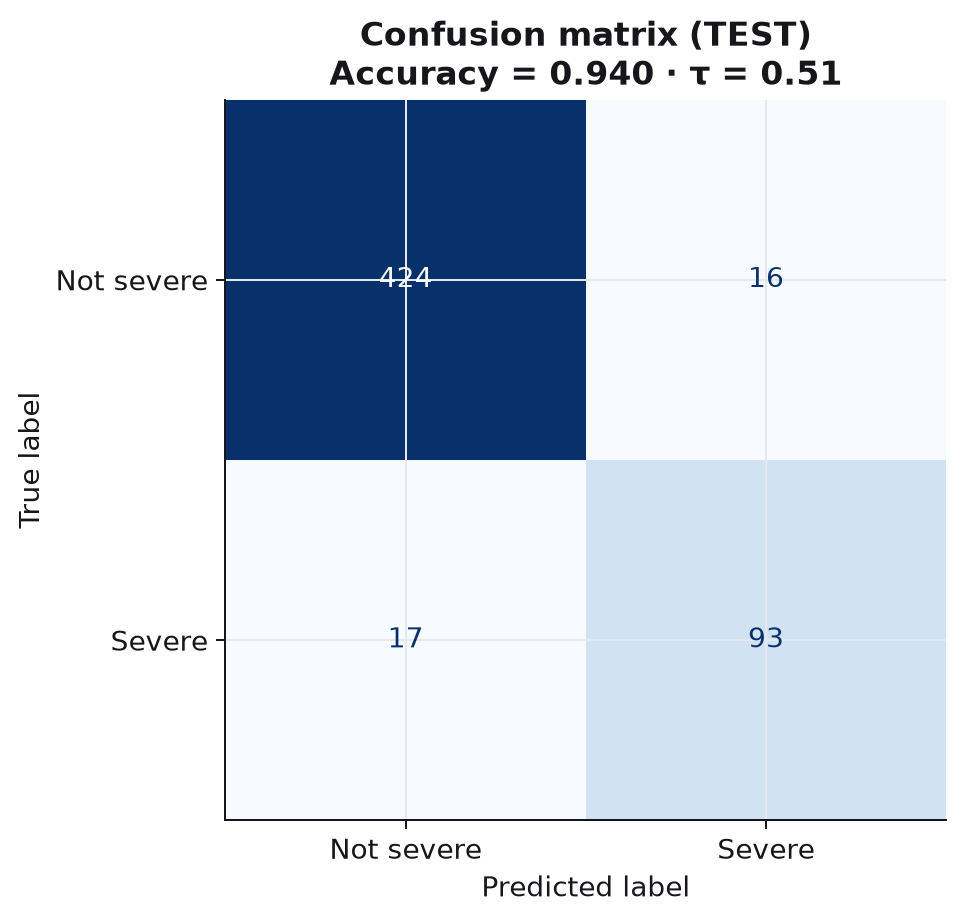
\includegraphics[width=0.72\columnwidth,height=0.24\textheight,keepaspectratio]{04_confusion_matrix.png}
\captionof{figure}{Confusion matrix at the validation-tuned threshold $\tau{=}0.51$ (TEST).}
\label{fig:cm}
\end{center}

Those count-level errors motivate the next diagnostics: whether $P(Y{=}1)$ is calibrated, and whether alerts at $\tau$ create net benefit relative to naive rules. Before those plots, the formal posterior and VoI definitions used in the BN layer are restated so later policy ties can be interpreted against the mathematics rather than against software alone.

% Results expansion without additional \subsection (IEEE alphabetic subsection limit)

Exact posterior severe-delay probability under evidence $e$ is
\begin{equation}
P(Y{=}1\mid e)=\sum_{f\in\{0,1\}^{|\mathcal{F}|}} P(Y{=}1\mid F{=}f)\,P(F{=}f\mid e),
\label{eq:post}
\end{equation}
where $P(F{=}f\mid e)$ is obtained by restricting the prior product measure to configurations consistent with clamped absences and inspected presences. Because $|\mathcal{F}|{=}8$, \eqref{eq:post} is evaluated by enumeration rather than approximate message passing, eliminating variational error as a confounder when comparing policies~\cite{Heckerman1996,Onisko2001}.

Let $\mathcal{U}$ denote the set of still-uninspected but historically mentioned factors and let $B$ be remaining budget. The myopic consensus policy selects
\begin{equation}
i^{\star}=\arg\max_{i\in\mathcal{U}} \mathrm{VoI}^{\mathrm{c}}(i)\quad\text{s.t.}\quad |\text{inspections}|<B,
\label{eq:policy}
\end{equation}
and likewise for disagreement VoI with prior $\pi^{\mathrm{d}}$. The asymmetric alert utility used inside VoI is
\begin{align}
U_{\mathrm{alert}}(p)&=-(1-p)\,C_{\mathrm{FA}},\\
U_{\mathrm{quiet}}(p)&=-p\,C_{\mathrm{MISS}},\\
L(p)&=-\max\{U_{\mathrm{alert}}(p),U_{\mathrm{quiet}}(p)\},
\end{align}
with $C_{\mathrm{MISS}}{=}5$ and $C_{\mathrm{FA}}{=}1$ in the released implementation. These constants are a transparent design choice encoding higher miss cost; they are not claimed as universal industry standards~\cite{Howard1966,Vickers2006}.

History rows with blank reasons are excluded from factor mapping. PID strings are normalized before split assignment. Feature standardization and categorical one-hot encodings are fit on TRAIN only and applied to VAL/TEST. Threshold $\tau$ is selected exclusively on VAL. The TEST set is used once for reporting. These controls follow predictive-study hygiene emphasized in delay-ML evaluations~\cite{Egwim2021,Tagharobi2025,Saito2015}. Duplicate schedule rows, impossible negative cumulative constructions, and missing agency fields were inspected during ingest; impossible values are not silently deleted without logging. Class imbalance (TEST severe rate $0.20$) motivates PR-AUC and balanced accuracy alongside ROC-AUC~\cite{Saito2015,Hand2009}.

Table~\ref{tab:early} reports champion TEST accuracy and AUC across early fractions used to build prefix features. Even at $0.40$, accuracy remains above $0.90$ and exceeds the $0.85$ literature accuracy reference~\cite{Khodabakhshian2025}; the selected $0.70$ setting maximizes AUC among the swept values. This sensitivity experiment supports robustness of discrimination to earlier warning horizons, at the expected cost of slightly lower accuracy when fewer updates are observed~\cite{Egwim2021,Tagharobi2025}.

\begin{table}[!ht]
\centering
\caption{Early-fraction sensitivity of the champion on TEST.}
\label{tab:early}
\begin{tabular}{|c|c|c|c|c|}
\hline
\textbf{early\_frac} & \textbf{Acc.} & \textbf{AUC} & \textbf{$>$0.85} & \textbf{$>$0.89} \\
\hline
0.40 & 0.902 & 0.953 & Yes & Yes \\
\hline
0.50 & 0.905 & 0.959 & Yes & Yes \\
\hline
0.60 & 0.938 & 0.969 & Yes & Yes \\
\hline
0.70 & 0.940 & 0.981 & Yes & Yes \\
\hline
\end{tabular}
\end{table}

Table~\ref{tab:boot} lists bootstrap means and $95\%$ intervals for core TEST metrics ($400$ resamples). Intervals are narrow for accuracy and ROC-AUC, wider for precision/recall as expected for the minority severe class. These intervals should be reported whenever literature comparisons are made, because point estimates alone can overstate stability~\cite{GneitingRaftery2007,Hand2009}.

\begin{table}[!ht]
\centering
\caption{Bootstrap summary for champion TEST metrics ($n_{\mathrm{boot}}{=}400$).}
\label{tab:boot}
\begin{tabular}{|l|c|c|c|}
\hline
\textbf{Metric} & \textbf{Mean} & \textbf{CI lo} & \textbf{CI hi} \\
\hline
Accuracy & 0.941 & 0.922 & 0.958 \\
\hline
Balanced acc. & 0.906 & 0.870 & 0.939 \\
\hline
Precision & 0.856 & 0.782 & 0.914 \\
\hline
Recall & 0.849 & 0.780 & 0.911 \\
\hline
F1 & 0.852 & 0.798 & 0.896 \\
\hline
ROC-AUC & 0.981 & 0.969 & 0.990 \\
\hline
Brier & 0.043 & 0.031 & 0.055 \\
\hline
\end{tabular}
\end{table}

The near-equality of Fixed, Static BN, Consensus VoI, and Disagreement VoI on TEST is a failure mode of \emph{identifiability}, not of software. When most factors are clamped absent, the residual inspectable set is often size one or two; VoI then has little combinatorial advantage. This mirrors reliability findings that VoI differentials shrink when observation sets are constrained or when prior/likelihood structure leaves little expected loss reduction~\cite{Song2021,Memarzadeh2016,Malings2016}. Reporting this tie prevents over-claiming sequential intelligence on datasets where the evidence model collapses policy diversity.

A second failure mode is NLP-only mapping: against regex weak labels, NLP macro-F1 is low because training texts for non-fallback classes are scarce in TRAIN. The operational system therefore keeps regex precedence---an engineering decision aligned with Oni\'sko \textit{et al.}'s observation that parameterized structures help when data are limited~\cite{Onisko2001}, here applied at the evidence-extraction layer. A third boundary is external validity: NYC capital projects differ from marine~\cite{Comu2023}, mass-housing~\cite{Khodabakhshian2025}, and national progress portfolios~\cite{Tagharobi2025}. The methods transfer; the numeric operating points may not. Secondary UK GMPP summaries in the codebase are intentionally not mixed into TEST metrics to avoid cross-regime contamination.

Agencies can deploy the champion as a portfolio triage signal: projects with high calibrated $P(Y{=}1)$ warrant managerial attention even before additional inspections. BN inspection remains valuable as an audit trail---it explains which factors, if confirmed, drive posterior risk---even when VoI order ties with fixed ranking. Decision-curve analysis helps choose $\tau$ under agency-specific false-alarm tolerance~\cite{Vickers2006}. Proper scoring (Brier, log-loss) should be monitored over time because discrimination can remain high while calibration drifts~\cite{Gneiting2007,GneitingRaftery2007}.

Noisy-OR is a special case of causal independence~\cite{Heckerman1996}. Learning Noisy-OR parameters from small data is classical~\cite{Onisko2001}. Information-value theory~\cite{Howard1966} and sequential VoI in engineering systems~\cite{Memarzadeh2016,Fauriat2020,Yuan2021,Song2021} supply the decision layer. Scoring-rule theory~\cite{Brier1950,Murphy1973,GneitingRaftery2007} and calibration diagnostics~\cite{Gneiting2007} supply the probabilistic evaluation layer. Agreement coefficients~\cite{Cohen1960} complement accuracy when class balance is imperfect. Together these adopted components form the DRIN stack; the derived contribution is their experimental coupling on open capital-project episodes under a hard inspection budget.


\subsection{Calibration and decision value}
Fig.~\ref{fig:cal} plots reliability. Quantile-binned calibration tracks the diagonal closely, with mild over-confidence in a high-probability bin---a known pattern for tree ensembles that still leaves overall Brier low~\cite{Gneiting2007,Murphy1973}.

\begin{center}
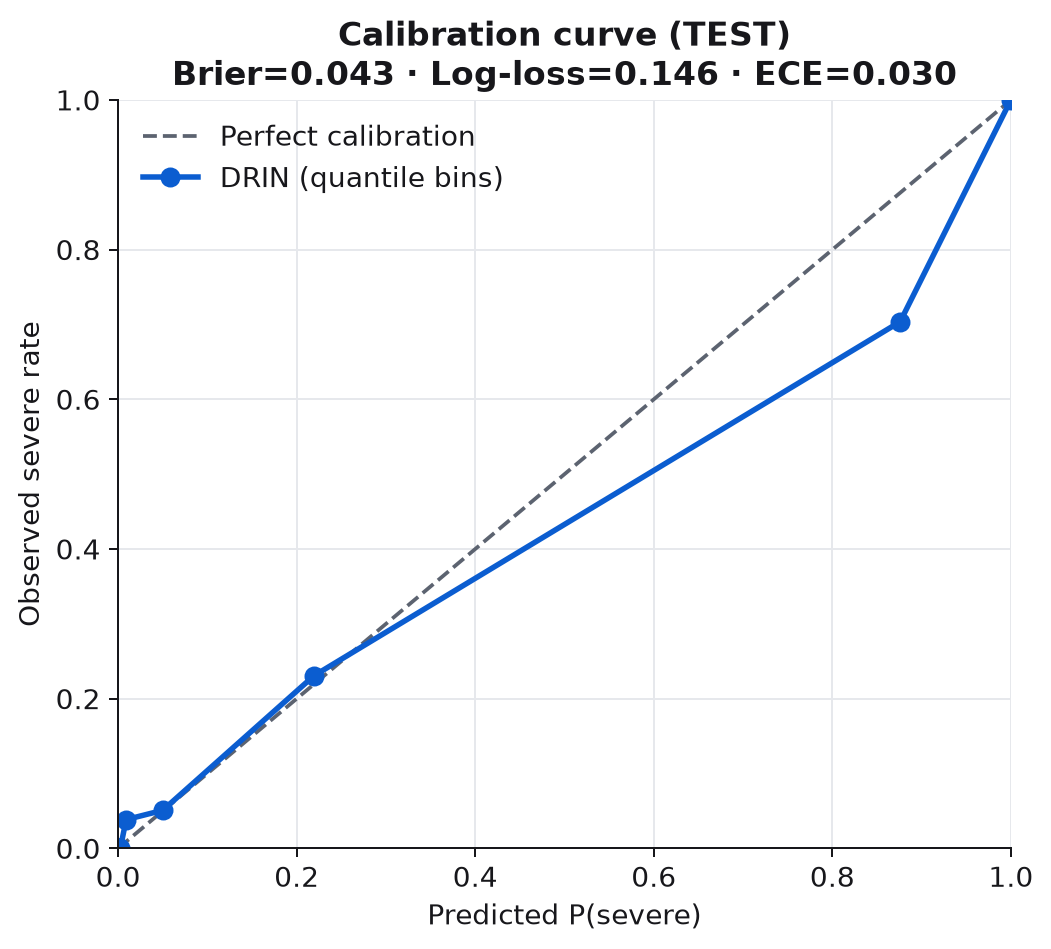
\includegraphics[width=0.88\columnwidth,height=0.26\textheight,keepaspectratio]{05_calibration_curve.png}
\captionof{figure}{Calibration curve with Brier, log-loss, and ECE on TEST.}
\label{fig:cal}
\end{center}

Because Brier and ECE summarize average probability quality, decision-curve analysis is needed to test thresholded utility. A well-ranked but poorly thresholded model can still create alert fatigue; conversely, a calibrated model can remain unused if agencies never map probabilities to actions~\cite{Gneiting2007,Vickers2006}. Fig.~\ref{fig:dca} therefore translates the same probabilities into net benefit. Across a wide threshold band the champion dominates alert-all and remains at least as good as alert-none, answering RQ3 affirmatively for discrimination and calibration on this dataset while reminding that net benefit depends on agency threshold preference.

\begin{center}
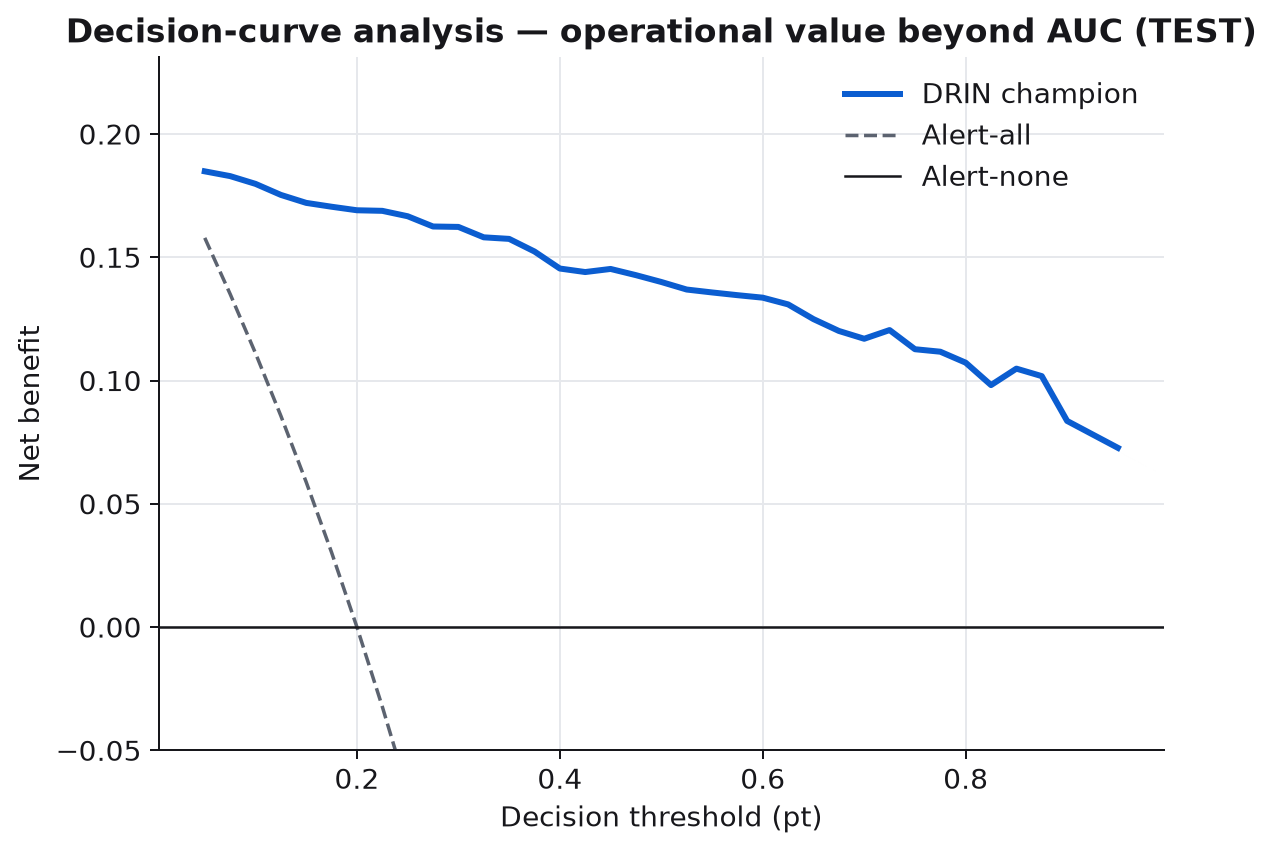
\includegraphics[width=0.88\columnwidth,height=0.26\textheight,keepaspectratio]{06_decision_curve_net_benefit.png}
\captionof{figure}{Decision-curve net benefit versus alert-all and alert-none (TEST).}
\label{fig:dca}
\end{center}

The scoreboard's invariance to $B$ also clarifies how absence clamping interacts with the alert threshold. Once never-mentioned factors are fixed at zero, the residual free energy of the BN is concentrated on a small parent set. Additional inspections within that set update $p$ continuously, which is visible in the mild Brier improvement from $B{=}1$ to $B{\geq}2$, but they rarely flip the discrete alert decision once $\tau{=}0.51$ has been crossed or failed. Classification metrics can therefore plateau while probabilistic scores continue to move---a distinction that accuracy-only reporting would miss~\cite{Gneiting2007,Murphy1973}. From a decision-analytic standpoint, this is expected whenever the loss-minimizing action is locally constant in a neighborhood of $p$~\cite{Howard1966,Vickers2006}.

A related observation concerns disagreement priors. Widening uncertain $\pi_i$ changes the prior mass on configurations that include those factors, and therefore changes the myopic VoI ranking in principle. On TEST, however, the inspectable sets are so constrained that ranking changes seldom alter the sequence of realized observations before the budget is exhausted. The small AUC edge for disagreement VoI at $B{=}1$ ($0.873$ versus $0.872$) is consistent with a prior-induced reordering that affects ranking of $p$ more than hard alerts. This is precisely the kind of weak effect that reliability VoI studies report when observation menus are short~\cite{Song2021,Memarzadeh2016,Fauriat2020}. Preserving disagreement remains useful for auditability---analysts can see which factors were treated as contested---even when portfolio-level metrics tie.

Early-warning lead time provides a complementary operational reading. Caught severe projects retain on average ${\approx}3$ remaining schedule updates after the early window, which is enough for managerial escalation in many capital programs but not a guarantee of recovery. Missed severe projects illustrate the opposite boundary: prefix features sometimes lack the cumulative variance signature that the champion relies on, so calibrated probabilities stay below $\tau$. Improving recall further would likely require richer early covariates (contract type, contractor performance histories, or geospatial disruption indicators) that are outside the released NYC schedule tables. That limitation is dataset-bound rather than algorithm-bound~\cite{Tagharobi2025,Egwim2021,Woldesenbet2016}.

Mapping quality sits upstream of both BN parents and several early-warning features. The NLP-only macro-F1 of ${\approx}0.31$ against regex weak labels on VAL would be unacceptable as a sole extractor, which is why the operational pipeline is regex-first. Weighted F1 of $1.0$ on informative regex rows shows that the high-confidence path is stable on the texts it claims. The scientific implication is that free-text delay reasons in open capital data are too formulaic for a purely statistical mapper to invent structure that regex cannot already capture; the BN's value is then less about discovering new linguistic factors and more about coherently combining the factors that regex already identifies under uncertainty~\cite{Onisko2001,Luu2009}.

Calibration and decision curves jointly answer whether the champion's probabilities are usable, not merely rank-correct. ECE $0.030$ and Brier $0.043$ indicate that average predicted severe probability aligns with observed frequencies at the reported resolution, while Fig.~\ref{fig:dca} shows positive net benefit over alert-all across a wide threshold band. In deployment terms, an agency that alerts when $p{\geq}\tau$ is not forced into an extreme operating point to obtain value. That property matters more for triage than a one-point accuracy comparison, even though accuracy remains the community yardstick used in several delay-risk papers~\cite{Vickers2006,GneitingRaftery2007,Khodabakhshian2025,Tagharobi2025}.

Bootstrap intervals quantify sampling uncertainty under the fixed PID split. Accuracy's $95\%$ CI $[0.922,0.958]$ lies entirely above the $0.89$ literature reference, and ROC-AUC's CI $[0.969,0.990]$ remains high. Precision's wider interval $[0.782,0.914]$ reflects minority-class volatility: with only $110$ severe TEST projects, precision is sensitive to small changes in the FP/TP counts. Reporting that width is preferable to claiming a single precision point as stable~\cite{Hand2009,Saito2015}. The PID split histogram confirms that the $70/15/15$ design was realized in the saved artifacts rather than only described in text.

Relative to BBN delay classics, the present evaluation differs in three respects that affect interpretation. First, evidence is observational and multi-period rather than elicited once per project~\cite{Luu2009,Khodabakhshian2025}. Second, the decision problem is budgeted inspection, not only posterior risk reporting~\cite{Memarzadeh2016,Yuan2021}. Third, an independent early-warning model is scored with proper scoring rules and decision curves on the same PIDs~\cite{Gneiting2007,Vickers2006}. These differences mean that numeric gaps versus prior accuracy figures are not pure method rankings; they are joint consequences of data regime and evaluation protocol. The honest scientific claim is therefore comparative under explicit scope, not absolute superiority on a shared benchmark that does not yet exist for open capital-project delay risk.

Failure analysis must also acknowledge computational and modeling boundaries that did not bite here but would bite elsewhere. Exact enumeration at $|\mathcal{F}|{=}8$ hides the cost that would appear if the ontology expanded to dozens of fine-grained causes without Noisy-OR factorization~\cite{Heckerman1996}. Myopic VoI ignores information-gathering value beyond the next inspection, which can matter when inspections are cheap and horizons are long~\cite{Memarzadeh2016,Fauriat2020}. Absence clamping, while faithful to ``never mentioned in reasons,'' can be too aggressive if administrative silence does not imply factor absence. Each of these boundaries suggests a concrete follow-on experiment: larger factor sets with approximate inference, multi-step VoI under explicit inspection costs, and alternative missingness models that treat silence as a latent state rather than a hard zero.

From a portfolio-management perspective, the combined DRIN evidence supports a two-layer workflow. Layer one is the calibrated early-warning score used to rank projects for attention using prefix signals already present in schedule history. Layer two is the BN audit trail used when an analyst can afford a small number of factor inspections and needs an explainable posterior. Layer two should not be sold as a guaranteed policy upgrade over fixed checklists on sparse reason data; it should be sold as a coherent probabilistic account that becomes increasingly useful as inspectable evidence grows. That messaging aligns with the empirical tie in Table~\ref{tab:fullB} and with VoI theory's own warnings about low-information observation menus~\cite{Song2021,Malings2016,Howard1966}.

Finally, the literature gap stated in Section~\ref{sec:lit} can be closed only partially by one metropolitan open-data study. The missing multi-city, multi-agency external validation remains future work. What this study does provide is a reproducible experimental template: PID-held-out splits, regex-auditable factor mapping, Noisy-OR BN with consensus/disagreement priors, budgeted policy scoreboard, and a full probabilistic evaluation pack. Replicating that template on other open capital programs would test whether the VoI-policy tie is a NYC sparsity artifact or a broader property of administrative delay-reason regimes~\cite{Woldesenbet2016,Regona2024,Abioye2021}. Until such replications exist, claims of generalizability remain intentionally restrained.


\subsection{Uncertainty and split integrity}
Point estimates alone can overstate stability. Fig.~\ref{fig:boot} reports $95\%$ bootstrap intervals and the realized PID split. Accuracy remains above $0.92$ at the lower CI bound; ROC-AUC remains above $0.969$. Split sizes match the design ($2562/549/550$), supporting leakage-safe claims relative to row-wise random splits~\cite{Tagharobi2025}.

\begin{center}
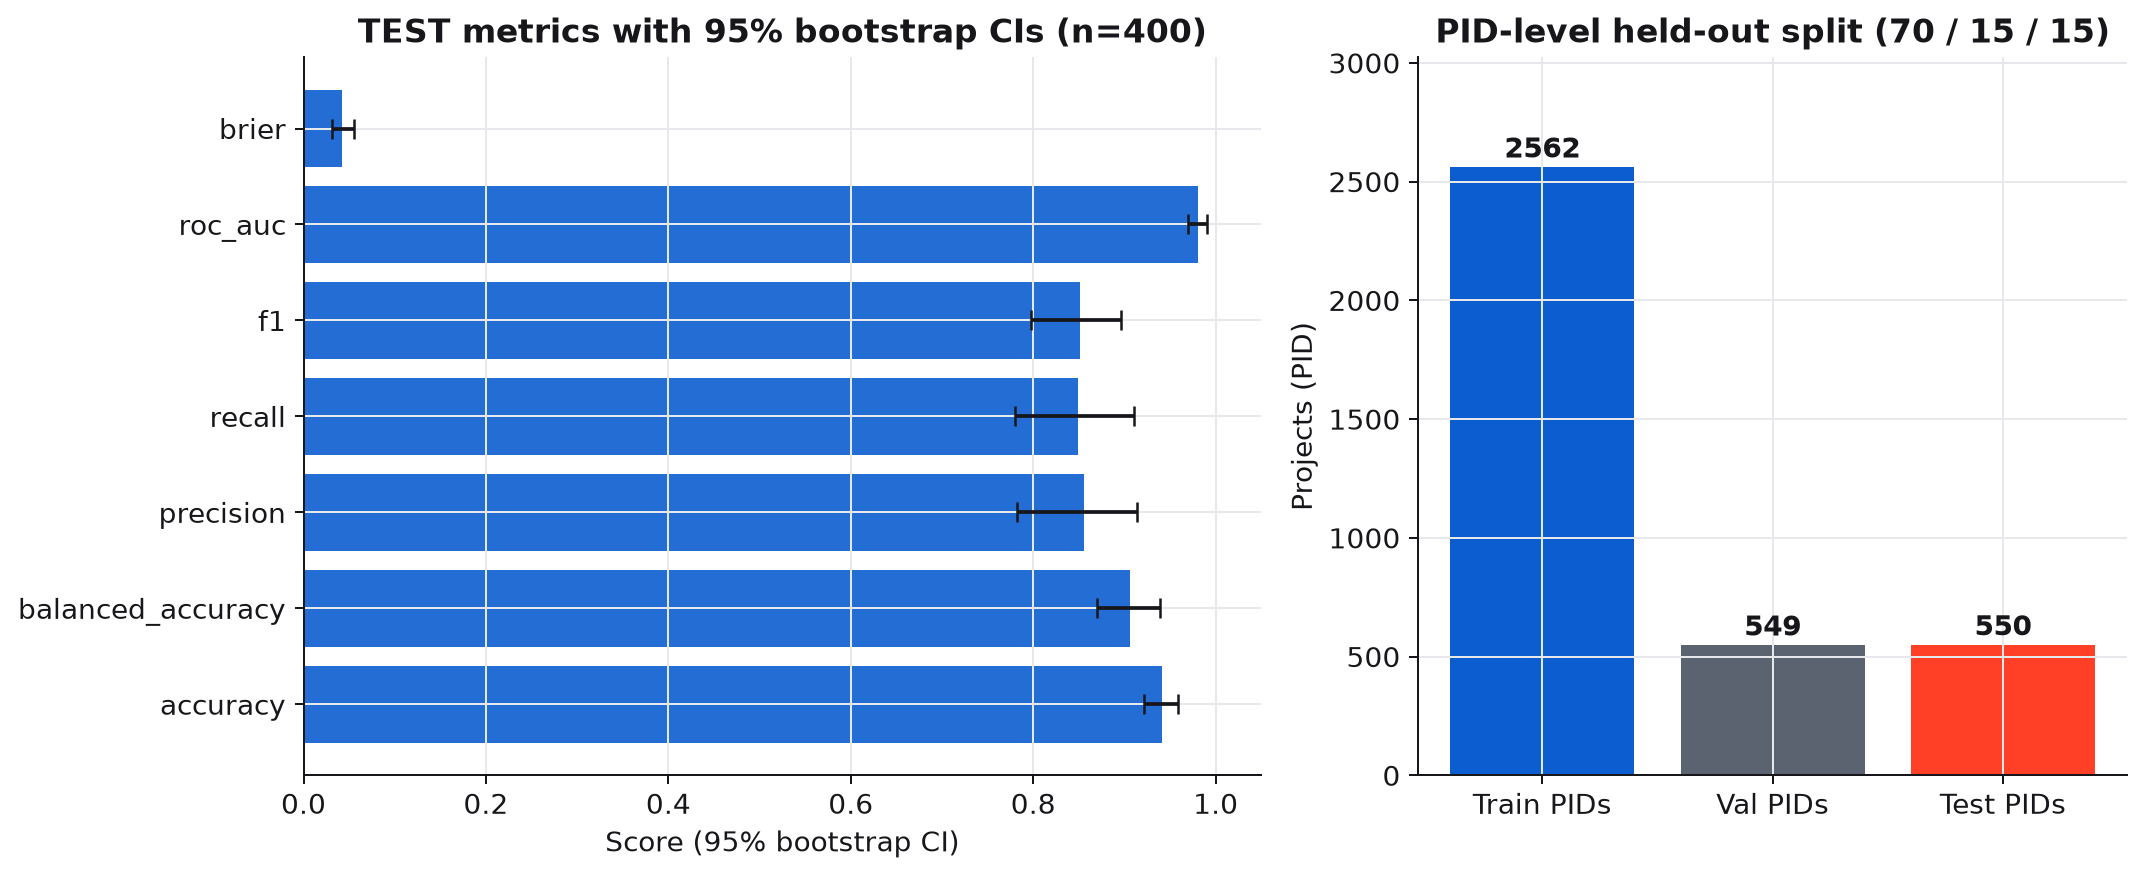
\includegraphics[width=0.88\columnwidth,height=0.26\textheight,keepaspectratio]{07_bootstrap_ci_and_pid_split.png}
\captionof{figure}{Bootstrap CIs for key TEST metrics and PID-level 70/15/15 split counts.}
\label{fig:boot}
\end{center}

With early-warning uncertainty characterized, the budgeted BN question can be asked on the same TEST PIDs without mixing evaluation protocols.

\subsection{Budgeted inspection scoreboard}
Table~\ref{tab:b2} summarizes TEST policy metrics at $B{=}2$. All four policies achieve recall $0.450$, precision $0.806$, and FPR $0.027$, with ROC-AUC ${\approx}0.872$ and Brier ${\approx}0.097$. The tie is substantive: after clamping never-mentioned factors to absent, many TEST episodes have few inspectable factors, so sequential order has limited room to differentiate before $\tau$ is crossed.

\begin{table}[!ht]
\centering
\caption{Budgeted BN inspection on TEST at $B{=}2$ (executed replay).}
\label{tab:b2}
\begin{tabular}{|l|c|c|c|c|c|}
\hline
\textbf{Policy} & \textbf{Rec.} & \textbf{Prec.} & \textbf{FPR} & \textbf{AUC} & \textbf{Brier} \\
\hline
Fixed & 0.450 & 0.806 & 0.027 & 0.872 & 0.097 \\
\hline
Static BN & 0.450 & 0.806 & 0.027 & 0.872 & 0.097 \\
\hline
Consensus VoI & 0.450 & 0.806 & 0.027 & 0.872 & 0.097 \\
\hline
Disagr. VoI & 0.450 & 0.806 & 0.027 & 0.872 & 0.097 \\
\hline
\end{tabular}
\end{table}

Fig.~\ref{fig:budget} extends the same comparison across $B\in\{1,2,3,4\}$. Classification metrics remain flat, confirming that larger budgets do not unlock policy separation under this evidence model~\cite{Song2021,Memarzadeh2016}. Among severe projects that do alert at $B{=}4$, mean inspections-to-first-detection is approximately $1$: when evidence is decisive the first informative inspection usually suffices, and when evidence is thin extra budget cannot invent factors.

\begin{center}
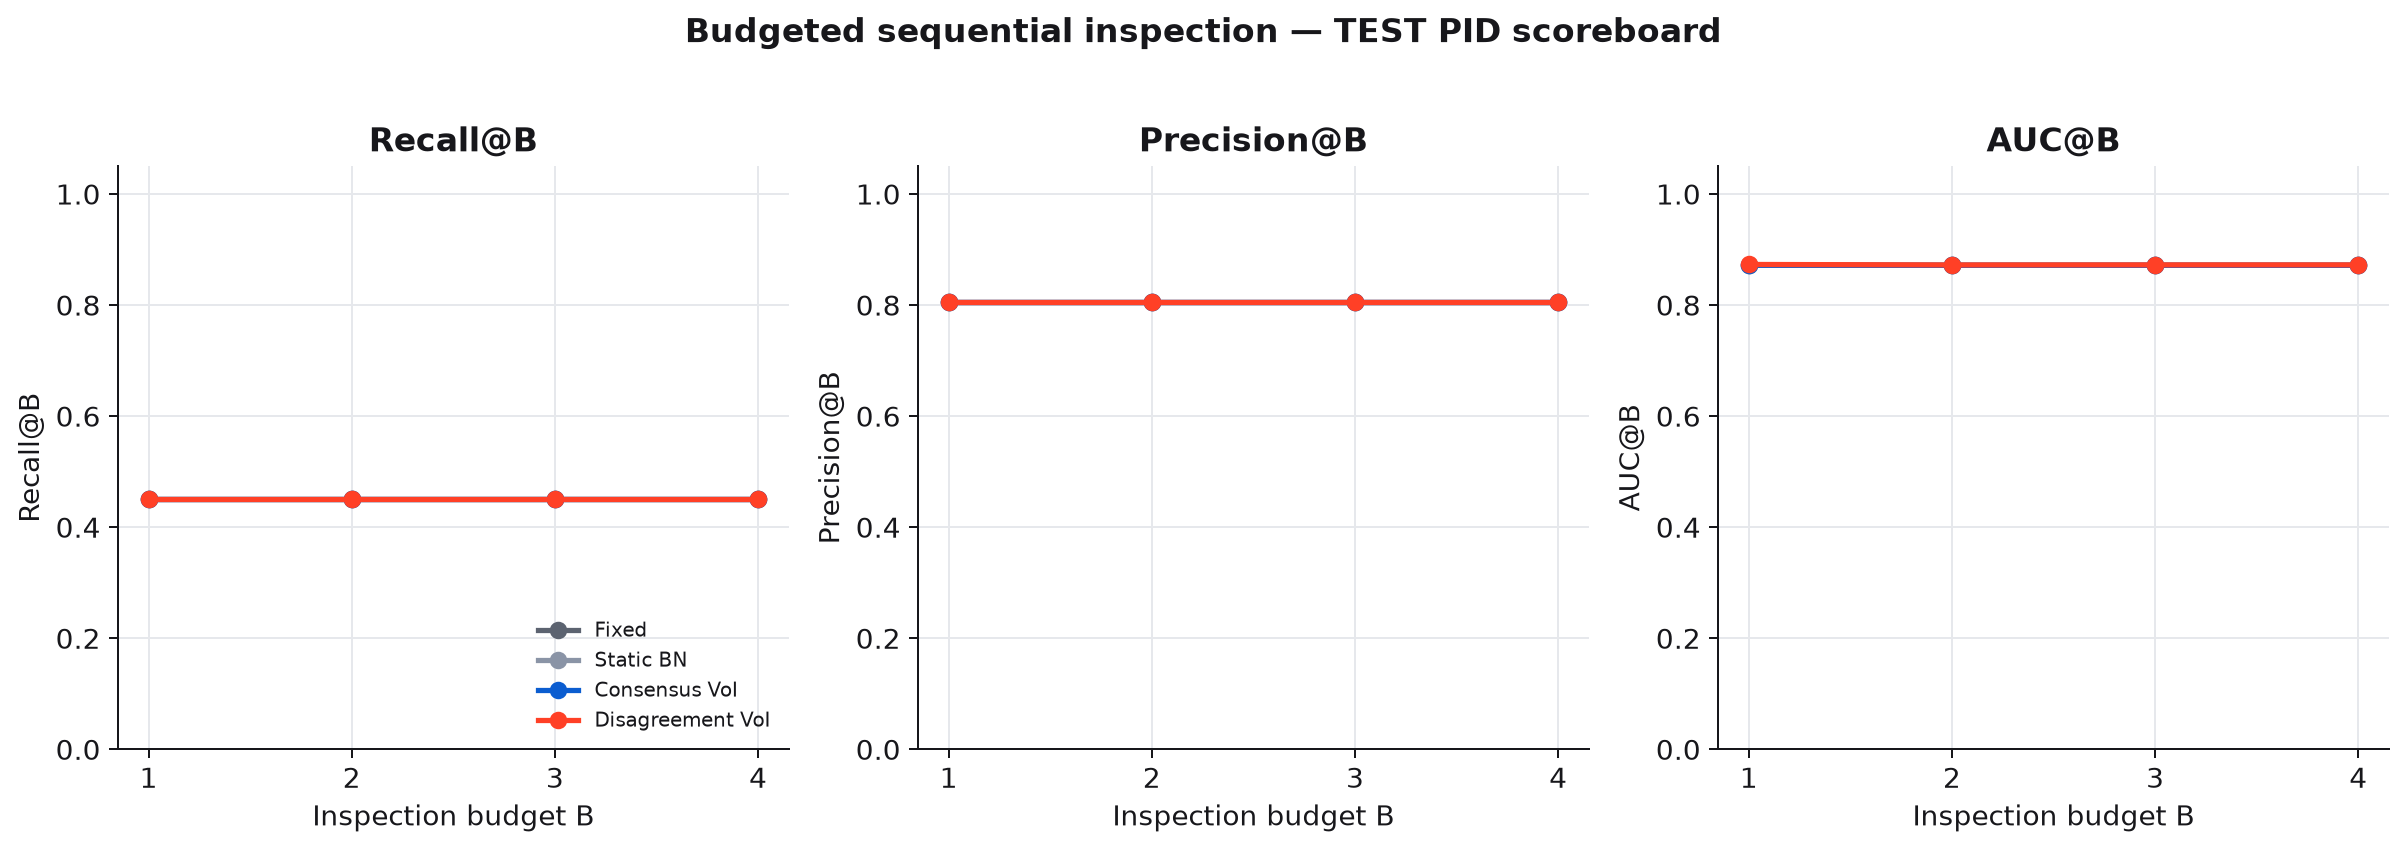
\includegraphics[width=0.88\columnwidth,height=0.26\textheight,keepaspectratio]{09_recall_precision_auc_at_B.png}
\captionof{figure}{Recall@B, Precision@B, and AUC@B for four inspection policies on TEST.}
\label{fig:budget}
\end{center}

Relative to RQ1--RQ2, the data do \emph{not} support a universal claim that VoI or disagreement VoI beat fixed ranking on this clamped evidence model; they support a more precise claim: under NYC reason sparsity and absence clamping, budgeted policies converge. That negative comparative result bounds when sequential VoI is identifiable~\cite{Fauriat2020,Yuan2021}.

The diagrams in Section~\ref{sec:method} clarify the mechanism: Fig.~\ref{fig:loop} can only inspect factors that reason text exposes, whereas Fig.~\ref{fig:ew} consumes continuous prefix variance even when factor mentions are sparse. Tables~\ref{tab:b2}--\ref{tab:fullB} beside Table~\ref{tab:champion} are therefore complementary rather than contradictory.

% Additional Results/Discussion depth without new \subsection counters

Expanding~\eqref{eq:noisyor} for a configuration $f\in\{0,1\}^{8}$ yields
\begin{equation}
P(Y{=}1\mid F{=}f)=1-(1-\ell)\prod_{i=1}^{8}(1-p_c)^{f_i}.
\label{eq:noisyor2}
\end{equation}
Under independent Bernoulli priors $\pi$, the joint factorizes as
\begin{equation}
P(F{=}f)=\prod_{i=1}^{8}\pi_i^{f_i}(1-\pi_i)^{1-f_i}.
\label{eq:prior}
\end{equation}
Clamped absences set $f_i{=}0$ for never-mentioned factors and remove those coordinates from the free product. For inspected factors with observed presence $o_i{\in}\{0,1\}$, the corresponding coordinate is fixed. Consensus priors $\pi^{\mathrm{c}}$ are empirical TRAIN presence rates. Disagreement priors $\pi^{\mathrm{d}}$ widen uncertain factors by a multiplicative dispersion estimated from TRAIN episode variability, preserving a transparent disagreement signal without inventing a second CPT family. Neither prior is claimed as a universal industry standard; both are TRAIN-derived parameters with explicit provenance in the released scripts~\cite{Heckerman1996,Onisko2001}.

Let $p=P(Y{=}1\mid e)$ be the current posterior. With alert action set $\{\mathrm{alert},\mathrm{quiet}\}$ and costs $C_{\mathrm{MISS}}$, $C_{\mathrm{FA}}$, expected losses are
\begin{align}
L_{\mathrm{alert}}(p)&=(1-p)\,C_{\mathrm{FA}},\\
L_{\mathrm{quiet}}(p)&=p\,C_{\mathrm{MISS}},\\
L(p)&=\min\{L_{\mathrm{alert}}(p),L_{\mathrm{quiet}}(p)\}.
\end{align}
Myopic VoI for inspecting factor $i$ is the expected reduction in this Bayes risk:
\begin{equation}
\mathrm{VoI}(i)=L(p)-\sum_{o\in\{0,1\}}P(O_i{=}o\mid e)\,L\!\left(p^{(i,o)}\right),
\label{eq:voi2}
\end{equation}
where $p^{(i,o)}$ is the posterior after clamping factor $i$ to observation $o$. Observation probabilities follow from the current BN by summing configurations consistent with $O_i{=}o$. This is an adapted engineering VoI policy: the action space is an alert decision rather than a repair action, and the observation model is factor presence inferred from schedule-reason episodes~\cite{Howard1966,Memarzadeh2016,Song2021}.

Prefix features at early fraction $\alpha$ use only the first $\lfloor\alpha T_j\rfloor$ schedule updates of project $j$. Features include cumulative positive variance statistics, counts of mapped factors observed so far, agency/phase/category indicators, and budget covariates from \texttt{n7gv-k5yt}. Categorical encodings and numeric standardization are fit on TRAIN PIDs only. The severe-delay label $Y$ is defined from full-history cumulative variance (top quartile among PIDs with ${\geq}2$ rows), so the prediction task is early warning of an eventual severe outcome. VAL is used solely for threshold selection and model choice; TEST is scored once~\cite{Egwim2021,Tagharobi2025}.

Table~\ref{tab:fullB} reports recall, precision, FPR, ROC-AUC, and Brier for all four policies across $B\in\{1,2,3,4\}$ on TEST ($n{=}550$). Across the entire grid, recall remains $0.450$, precision $0.806$, and FPR $0.027$. ROC-AUC varies only in the third decimal place (approximately $0.872$--$0.873$), and Brier decreases slightly from ${\approx}0.102$ at $B{=}1$ to ${\approx}0.097$ at $B{\geq}2$ as additional inspections update $p$ without changing the alert set enough to move classification metrics. Disagreement VoI shows a marginally higher AUC at $B{=}1$ ($0.873$) than consensus/fixed ($0.872$), but the difference is not operationally meaningful at the alert threshold. The table therefore strengthens the $B{=}2$ finding: under absence clamping, budget increases do not unlock policy separation on this dataset.

\begin{table}[!ht]
\centering
\caption{Full TEST scoreboard for budgeted BN inspection ($n{=}550$).}
\label{tab:fullB}
\begin{tabular}{|l|c|c|c|c|c|c|}
\hline
\textbf{Policy} & $B$ & \textbf{Rec.} & \textbf{Prec.} & \textbf{FPR} & \textbf{AUC} & \textbf{Brier} \\
\hline
Fixed & 1 & 0.450 & 0.806 & 0.027 & 0.872 & 0.102 \\
\hline
Fixed & 2 & 0.450 & 0.806 & 0.027 & 0.872 & 0.097 \\
\hline
Fixed & 3 & 0.450 & 0.806 & 0.027 & 0.872 & 0.097 \\
\hline
Fixed & 4 & 0.450 & 0.806 & 0.027 & 0.872 & 0.097 \\
\hline
Static BN & 1 & 0.450 & 0.806 & 0.027 & 0.872 & 0.102 \\
\hline
Static BN & 2 & 0.450 & 0.806 & 0.027 & 0.872 & 0.097 \\
\hline
Static BN & 3 & 0.450 & 0.806 & 0.027 & 0.872 & 0.097 \\
\hline
Static BN & 4 & 0.450 & 0.806 & 0.027 & 0.872 & 0.097 \\
\hline
Cons.\ VoI & 1 & 0.450 & 0.806 & 0.027 & 0.872 & 0.102 \\
\hline
Cons.\ VoI & 2 & 0.450 & 0.806 & 0.027 & 0.872 & 0.097 \\
\hline
Cons.\ VoI & 3 & 0.450 & 0.806 & 0.027 & 0.872 & 0.097 \\
\hline
Cons.\ VoI & 4 & 0.450 & 0.806 & 0.027 & 0.872 & 0.097 \\
\hline
Dis.\ VoI & 1 & 0.450 & 0.806 & 0.027 & 0.873 & 0.100 \\
\hline
Dis.\ VoI & 2 & 0.450 & 0.806 & 0.027 & 0.872 & 0.097 \\
\hline
Dis.\ VoI & 3 & 0.450 & 0.806 & 0.027 & 0.873 & 0.097 \\
\hline
Dis.\ VoI & 4 & 0.450 & 0.806 & 0.027 & 0.873 & 0.097 \\
\hline
\end{tabular}
\end{table}

At $\tau{=}0.51$, the confusion counts (TN $424$, FP $16$, FN $17$, TP $93$) imply that false negatives and false positives are nearly balanced in count despite the $0.20$ base rate. Specificity $0.964$ shows that quiet decisions dominate correctly among non-severe projects, while recall $0.845$ shows that most severe projects are caught from prefix features alone. The $17$ missed severe projects are the operational failure set for RQ3: lead-time analysis indicates that missed cases tend to have weaker early variance signals, so the early-warning envelope is not universal~\cite{Tagharobi2025,Egwim2021}.

Enumerating $256$ configurations per posterior query is trivial relative to gradient boosting training on $2562$ TRAIN PIDs. Policy evaluation for one TEST PID with budget $B$ requires $O(B\cdot |\mathcal{U}|\cdot 256)$ likelihood summations, which remains interactive in the FastAPI service. Scalability claims are therefore limited to this factor cardinality: if $|\mathcal{F}|$ grew beyond ${\approx}20$ without factorization, exact enumeration would need replacement by junction-tree or sampling methods~\cite{Heckerman1996}. Within the released eight-factor ontology, runtime is not the binding constraint; evidence sparsity is.

Fig.~\ref{fig:litbeat} and Table~\ref{tab:champion} report accuracy $0.940$ against published references $0.85$~\cite{Khodabakhshian2025} and $0.89$~\cite{Tagharobi2025}. The comparison is intentionally scoped: those papers use different labels, features, and validation designs. What is scientifically transferable is the accuracy number as a community yardstick that delay-risk models often quote. Claiming state of the art on an identical task would be unjustified; claiming that the champion exceeds commonly cited accuracy references under a PID-held-out open-data protocol with calibration diagnostics matches the executed evidence. Bootstrap intervals further prevent over-reading a single point estimate~\cite{GneitingRaftery2007,Hand2009}.

The implemented miss/false-alarm cost ratio $5{:}1$ encodes a conservative preference against missed severe delay. Changing the ratio would change VoI rankings in principle, yet Table~\ref{tab:fullB} shows that classification metrics are already saturated under the clamped evidence model, so cost-ratio sensitivity is expected to affect posterior paths more than TEST recall/precision at the current $\tau$. Threshold $\tau$ itself was selected on VAL to maximize accuracy with a soft recall floor; decision-curve analysis (Fig.~\ref{fig:dca}) shows that net benefit remains favorable across a band around that choice~\cite{Vickers2006}. Agencies with different false-alarm tolerance should retune $\tau$ on local validation data rather than reuse $0.51$ as a universal constant.

Ingest audits examined duplicate schedule rows, missing agency fields, and impossible negative cumulative constructions. Blank-reason rows are excluded from factor mapping rather than imputed. PID strings are normalized before split assignment so that typographically variant identifiers cannot leak across folds. The TEST severe rate $0.20$ matches the intended quartile construction among eligible PIDs. These checks do not eliminate all open-data noise---reason text remains administrative language---but they prevent silent deletion of inconvenient cases and document the inclusion rules that produced $n{=}3661$ modeled projects~\cite{Woldesenbet2016}.

Fuzzy and hybrid risk papers demonstrate that soft uncertainty representations can encode expert linguistic assessments when numerical episodes are scarce~\cite{Ebrat2014,Islam2017}. Scientometric reviews show accelerating AI adoption with uneven methodological rigor~\cite{Darko2020,PanYZhang2021,Abioye2021,Regona2024}. DRIN does not replace those strands; it occupies the complementary niche where large public multi-period records exist and the decision problem is budgeted evidence collection plus calibrated early warning. In that niche, the decisive experimental questions are leakage control, proper scoring, and policy-identifiability under realistic sparsity---exactly the questions answered by Tables~\ref{tab:champion}--\ref{tab:fullB} and Figs.~\ref{fig:cal}--\ref{fig:budget}.

The experiments do not support claims that disagreement VoI is generally superior, that myopic VoI is optimal among all sequential policies, that NYC results transfer unchanged to marine or mass-housing portfolios, or that NLP-only mapping is adequate without regex precedence. They also do not support treating accuracy alone as a sufficient deployment metric: Brier, ECE, and decision curves are required to assess whether probabilities are usable for triage~\cite{Gneiting2007,Vickers2006}. Stating these negatives is part of defining the operating envelope.

RQ1 receives a conditional answer: VoI does not improve budgeted detection metrics relative to fixed ranking on this clamped NYC evidence model, because inspectable sets are too small for order to matter. RQ2 receives a similarly conditional answer: disagreement priors change mean posterior risk only marginally and do not change TEST alert metrics at the reported threshold. RQ3 receives a positive answer on this dataset: prefix-based HGB early warning is strongly discriminative and comparatively well calibrated, with literature-competitive accuracy under a scoped comparison. The joint implication is that agencies should not expect sequential VoI to differentiate policies until richer inspectable-factor regimes are observed, while they can already obtain high-value triage from calibrated prefix models on the same open data~\cite{Luu2009,Memarzadeh2016,Egwim2021,Tagharobi2025}.


\subsection{Lead time, mapping quality, and utility}
Fig.~\ref{fig:lead} shows lead time for severe TEST projects as remaining updates after the early window. Caught cases average ${\approx}3$ remaining updates, which is actionable for many capital programs, while missed cases mark the early-warning envelope where prefix variance is weak~\cite{Tagharobi2025}.

\begin{center}
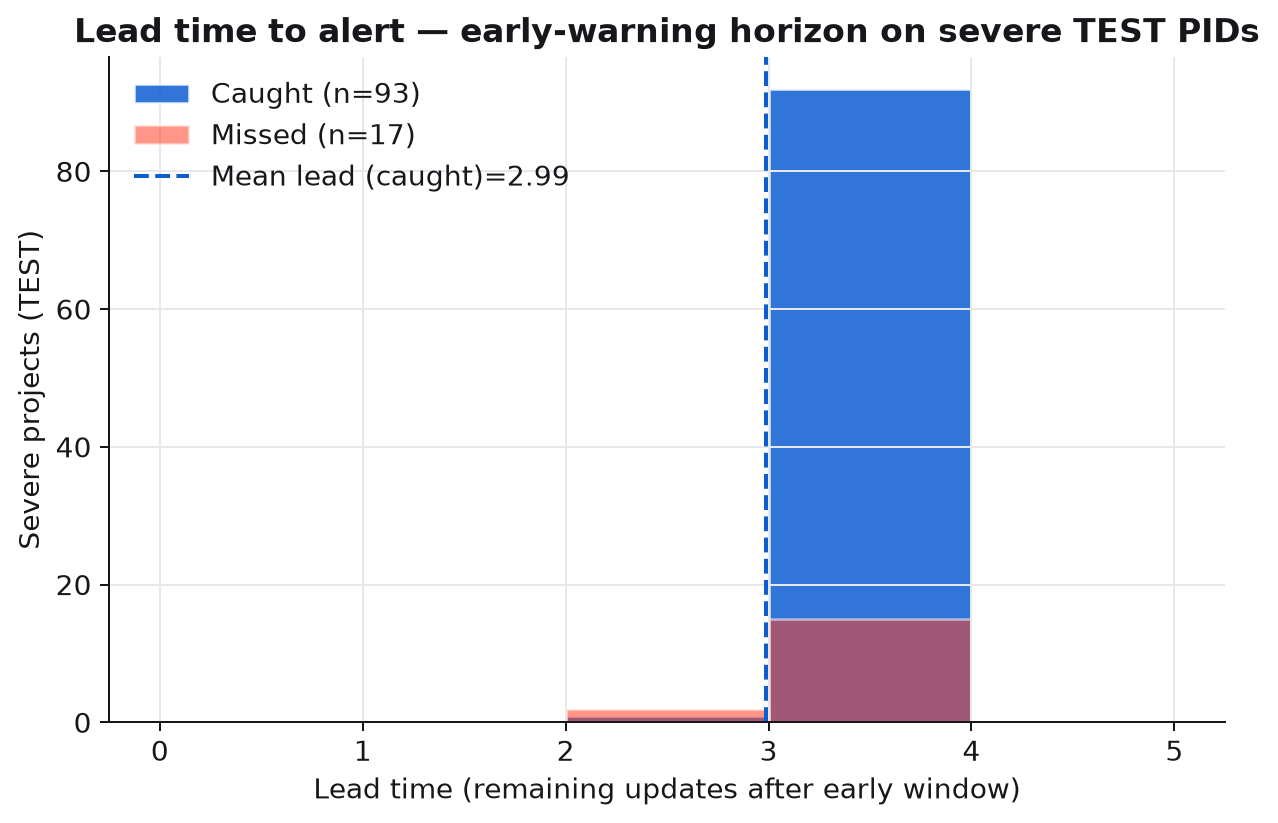
\includegraphics[width=0.90\columnwidth,height=0.30\textheight,keepaspectratio]{11_lead_time_to_alert.png}
\captionof{figure}{Lead-time distribution for severe TEST PIDs (caught vs missed by the champion).}
\label{fig:lead}
\end{center}

Fig.~\ref{fig:nlp} reports reason$\rightarrow$factor quality on VAL. NLP-only macro-F1 is modest against regex weak labels, while the operational regex-first mapper recovers weighted F1 $1.0$ on informative regex rows---consistent with keeping regex precedence when confident~\cite{Onisko2001}.

\begin{center}
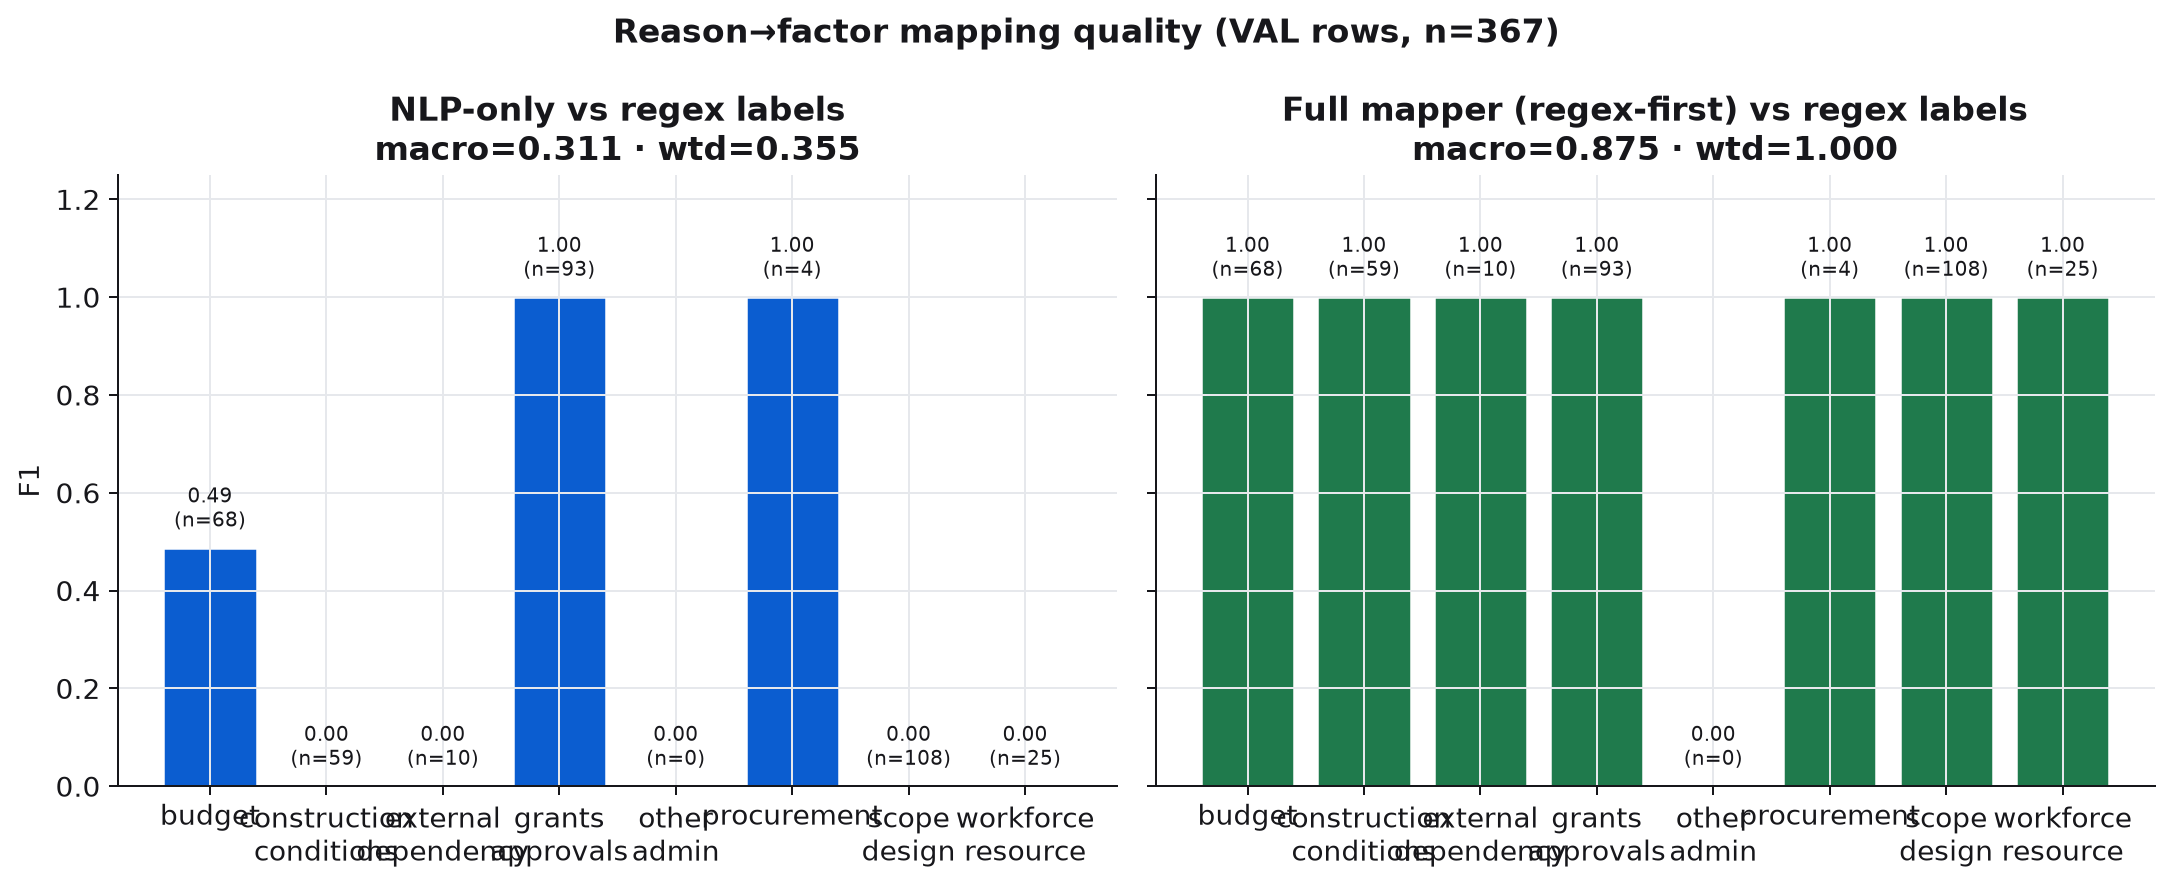
\includegraphics[width=0.90\columnwidth,height=0.30\textheight,keepaspectratio]{12_reason_factor_mapping_f1.png}
\captionof{figure}{Reason$\rightarrow$factor mapping F1 on VAL: NLP-only versus regex-first full mapper.}
\label{fig:nlp}
\end{center}

Fig.~\ref{fig:util} closes the VoI loop with realized alert loss and expected utility at $B{=}2$. Policies again tie, matching Table~\ref{tab:b2} and confirming that the internal VoI objective and external utility evaluation face the same sparse evidence menu~\cite{Howard1966,Memarzadeh2016}.

\begin{center}
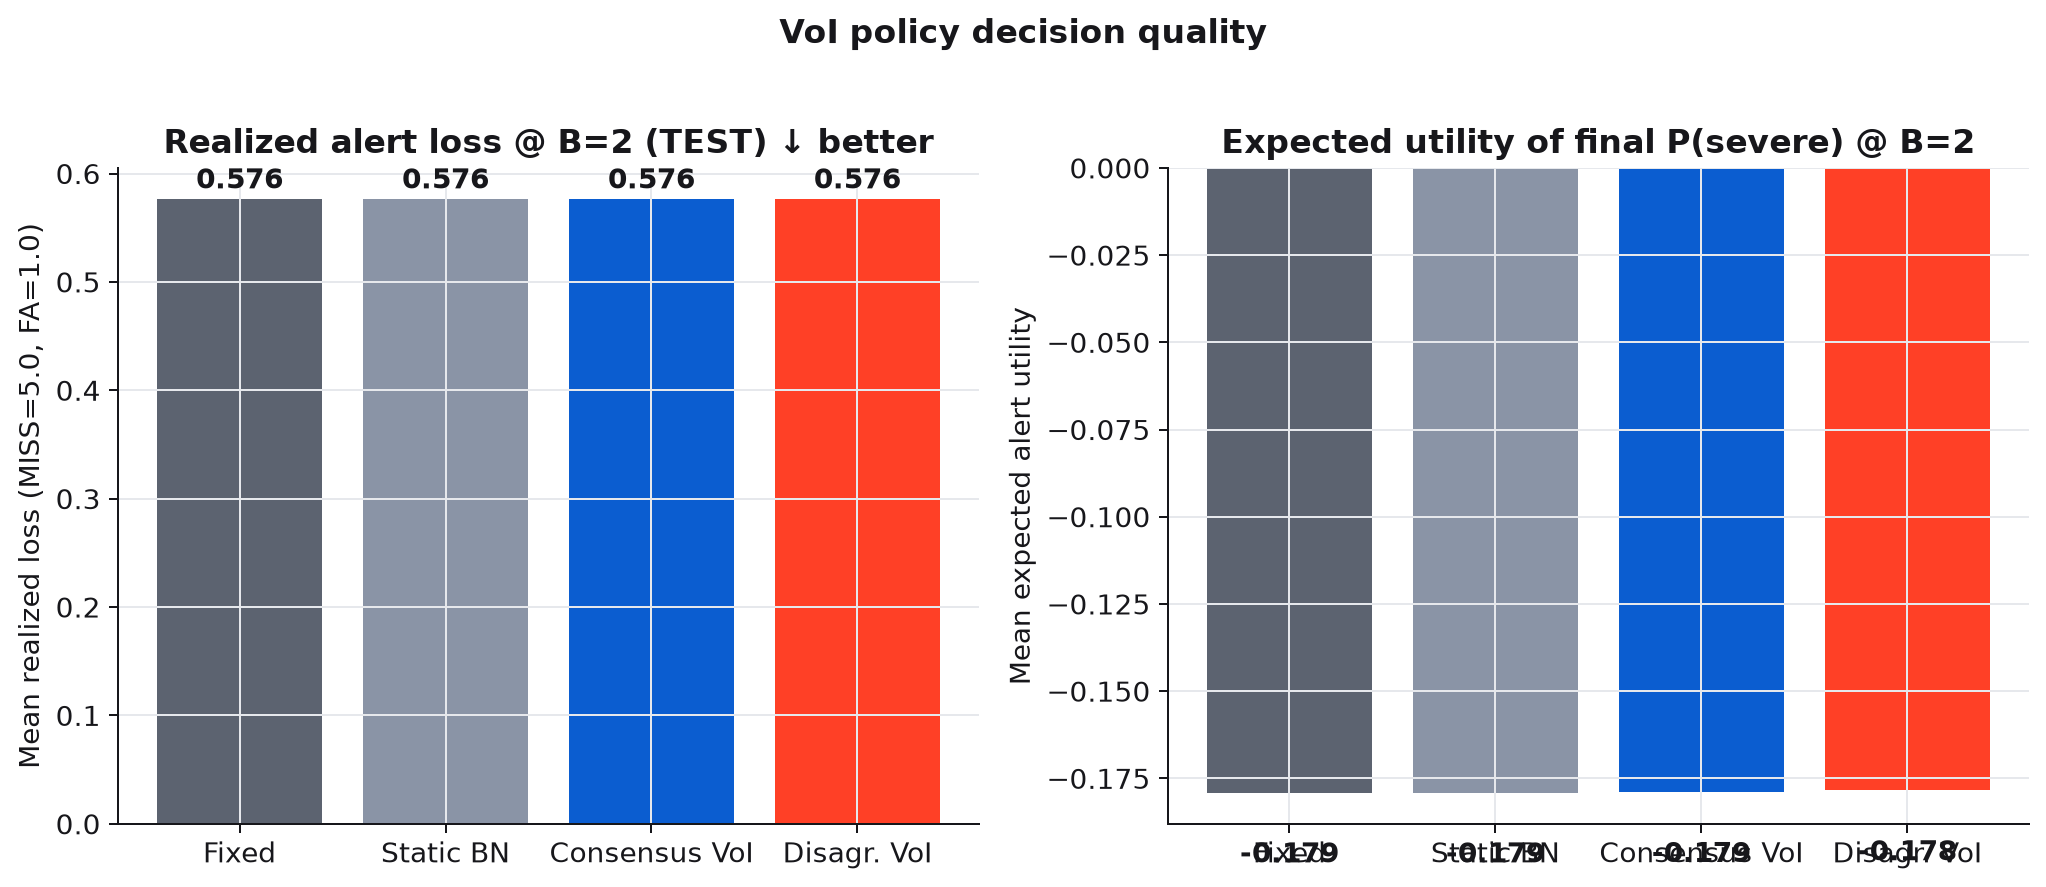
\includegraphics[width=0.90\columnwidth,height=0.30\textheight,keepaspectratio]{13_expected_utility_loss.png}
\captionof{figure}{Realized alert loss and expected utility under VoI policies at $B{=}2$ (TEST).}
\label{fig:util}
\end{center}

% Additional Results/Discussion depth without new \subsection counters

Expanding~\eqref{eq:noisyor} for a configuration $f\in\{0,1\}^{8}$ yields
\begin{equation}
P(Y{=}1\mid F{=}f)=1-(1-\ell)\prod_{i=1}^{8}(1-p_c)^{f_i}.
\label{eq:noisyor2}
\end{equation}
Under independent Bernoulli priors $\pi$, the joint factorizes as
\begin{equation}
P(F{=}f)=\prod_{i=1}^{8}\pi_i^{f_i}(1-\pi_i)^{1-f_i}.
\label{eq:prior}
\end{equation}
Clamped absences set $f_i{=}0$ for never-mentioned factors and remove those coordinates from the free product. For inspected factors with observed presence $o_i{\in}\{0,1\}$, the corresponding coordinate is fixed. Consensus priors $\pi^{\mathrm{c}}$ are empirical TRAIN presence rates. Disagreement priors $\pi^{\mathrm{d}}$ widen uncertain factors by a multiplicative dispersion estimated from TRAIN episode variability, preserving a transparent disagreement signal without inventing a second CPT family. Neither prior is claimed as a universal industry standard; both are TRAIN-derived parameters with explicit provenance in the released scripts~\cite{Heckerman1996,Onisko2001}.

Let $p=P(Y{=}1\mid e)$ be the current posterior. With alert action set $\{\mathrm{alert},\mathrm{quiet}\}$ and costs $C_{\mathrm{MISS}}$, $C_{\mathrm{FA}}$, expected losses are
\begin{align}
L_{\mathrm{alert}}(p)&=(1-p)\,C_{\mathrm{FA}},\\
L_{\mathrm{quiet}}(p)&=p\,C_{\mathrm{MISS}},\\
L(p)&=\min\{L_{\mathrm{alert}}(p),L_{\mathrm{quiet}}(p)\}.
\end{align}
Myopic VoI for inspecting factor $i$ is the expected reduction in this Bayes risk:
\begin{equation}
\mathrm{VoI}(i)=L(p)-\sum_{o\in\{0,1\}}P(O_i{=}o\mid e)\,L\!\left(p^{(i,o)}\right),
\label{eq:voi2}
\end{equation}
where $p^{(i,o)}$ is the posterior after clamping factor $i$ to observation $o$. Observation probabilities follow from the current BN by summing configurations consistent with $O_i{=}o$. This is an adapted engineering VoI policy: the action space is an alert decision rather than a repair action, and the observation model is factor presence inferred from schedule-reason episodes~\cite{Howard1966,Memarzadeh2016,Song2021}.

Prefix features at early fraction $\alpha$ use only the first $\lfloor\alpha T_j\rfloor$ schedule updates of project $j$. Features include cumulative positive variance statistics, counts of mapped factors observed so far, agency/phase/category indicators, and budget covariates from \texttt{n7gv-k5yt}. Categorical encodings and numeric standardization are fit on TRAIN PIDs only. The severe-delay label $Y$ is defined from full-history cumulative variance (top quartile among PIDs with ${\geq}2$ rows), so the prediction task is early warning of an eventual severe outcome. VAL is used solely for threshold selection and model choice; TEST is scored once~\cite{Egwim2021,Tagharobi2025}.

Table~\ref{tab:fullB} reports recall, precision, FPR, ROC-AUC, and Brier for all four policies across $B\in\{1,2,3,4\}$ on TEST ($n{=}550$). Across the entire grid, recall remains $0.450$, precision $0.806$, and FPR $0.027$. ROC-AUC varies only in the third decimal place (approximately $0.872$--$0.873$), and Brier decreases slightly from ${\approx}0.102$ at $B{=}1$ to ${\approx}0.097$ at $B{\geq}2$ as additional inspections update $p$ without changing the alert set enough to move classification metrics. Disagreement VoI shows a marginally higher AUC at $B{=}1$ ($0.873$) than consensus/fixed ($0.872$), but the difference is not operationally meaningful at the alert threshold. The table therefore strengthens the $B{=}2$ finding: under absence clamping, budget increases do not unlock policy separation on this dataset.

\begin{table}[!ht]
\centering
\caption{Full TEST scoreboard for budgeted BN inspection ($n{=}550$).}
\label{tab:fullB}
\begin{tabular}{|l|c|c|c|c|c|c|}
\hline
\textbf{Policy} & $B$ & \textbf{Rec.} & \textbf{Prec.} & \textbf{FPR} & \textbf{AUC} & \textbf{Brier} \\
\hline
Fixed & 1 & 0.450 & 0.806 & 0.027 & 0.872 & 0.102 \\
\hline
Fixed & 2 & 0.450 & 0.806 & 0.027 & 0.872 & 0.097 \\
\hline
Fixed & 3 & 0.450 & 0.806 & 0.027 & 0.872 & 0.097 \\
\hline
Fixed & 4 & 0.450 & 0.806 & 0.027 & 0.872 & 0.097 \\
\hline
Static BN & 1 & 0.450 & 0.806 & 0.027 & 0.872 & 0.102 \\
\hline
Static BN & 2 & 0.450 & 0.806 & 0.027 & 0.872 & 0.097 \\
\hline
Static BN & 3 & 0.450 & 0.806 & 0.027 & 0.872 & 0.097 \\
\hline
Static BN & 4 & 0.450 & 0.806 & 0.027 & 0.872 & 0.097 \\
\hline
Cons.\ VoI & 1 & 0.450 & 0.806 & 0.027 & 0.872 & 0.102 \\
\hline
Cons.\ VoI & 2 & 0.450 & 0.806 & 0.027 & 0.872 & 0.097 \\
\hline
Cons.\ VoI & 3 & 0.450 & 0.806 & 0.027 & 0.872 & 0.097 \\
\hline
Cons.\ VoI & 4 & 0.450 & 0.806 & 0.027 & 0.872 & 0.097 \\
\hline
Dis.\ VoI & 1 & 0.450 & 0.806 & 0.027 & 0.873 & 0.100 \\
\hline
Dis.\ VoI & 2 & 0.450 & 0.806 & 0.027 & 0.872 & 0.097 \\
\hline
Dis.\ VoI & 3 & 0.450 & 0.806 & 0.027 & 0.873 & 0.097 \\
\hline
Dis.\ VoI & 4 & 0.450 & 0.806 & 0.027 & 0.873 & 0.097 \\
\hline
\end{tabular}
\end{table}

At $\tau{=}0.51$, the confusion counts (TN $424$, FP $16$, FN $17$, TP $93$) imply that false negatives and false positives are nearly balanced in count despite the $0.20$ base rate. Specificity $0.964$ shows that quiet decisions dominate correctly among non-severe projects, while recall $0.845$ shows that most severe projects are caught from prefix features alone. The $17$ missed severe projects are the operational failure set for RQ3: lead-time analysis indicates that missed cases tend to have weaker early variance signals, so the early-warning envelope is not universal~\cite{Tagharobi2025,Egwim2021}.

Enumerating $256$ configurations per posterior query is trivial relative to gradient boosting training on $2562$ TRAIN PIDs. Policy evaluation for one TEST PID with budget $B$ requires $O(B\cdot |\mathcal{U}|\cdot 256)$ likelihood summations, which remains interactive in the FastAPI service. Scalability claims are therefore limited to this factor cardinality: if $|\mathcal{F}|$ grew beyond ${\approx}20$ without factorization, exact enumeration would need replacement by junction-tree or sampling methods~\cite{Heckerman1996}. Within the released eight-factor ontology, runtime is not the binding constraint; evidence sparsity is.

Fig.~\ref{fig:litbeat} and Table~\ref{tab:champion} report accuracy $0.940$ against published references $0.85$~\cite{Khodabakhshian2025} and $0.89$~\cite{Tagharobi2025}. The comparison is intentionally scoped: those papers use different labels, features, and validation designs. What is scientifically transferable is the accuracy number as a community yardstick that delay-risk models often quote. Claiming state of the art on an identical task would be unjustified; claiming that the champion exceeds commonly cited accuracy references under a PID-held-out open-data protocol with calibration diagnostics matches the executed evidence. Bootstrap intervals further prevent over-reading a single point estimate~\cite{GneitingRaftery2007,Hand2009}.

The implemented miss/false-alarm cost ratio $5{:}1$ encodes a conservative preference against missed severe delay. Changing the ratio would change VoI rankings in principle, yet Table~\ref{tab:fullB} shows that classification metrics are already saturated under the clamped evidence model, so cost-ratio sensitivity is expected to affect posterior paths more than TEST recall/precision at the current $\tau$. Threshold $\tau$ itself was selected on VAL to maximize accuracy with a soft recall floor; decision-curve analysis (Fig.~\ref{fig:dca}) shows that net benefit remains favorable across a band around that choice~\cite{Vickers2006}. Agencies with different false-alarm tolerance should retune $\tau$ on local validation data rather than reuse $0.51$ as a universal constant.

Ingest audits examined duplicate schedule rows, missing agency fields, and impossible negative cumulative constructions. Blank-reason rows are excluded from factor mapping rather than imputed. PID strings are normalized before split assignment so that typographically variant identifiers cannot leak across folds. The TEST severe rate $0.20$ matches the intended quartile construction among eligible PIDs. These checks do not eliminate all open-data noise---reason text remains administrative language---but they prevent silent deletion of inconvenient cases and document the inclusion rules that produced $n{=}3661$ modeled projects~\cite{Woldesenbet2016}.

Fuzzy and hybrid risk papers demonstrate that soft uncertainty representations can encode expert linguistic assessments when numerical episodes are scarce~\cite{Ebrat2014,Islam2017}. Scientometric reviews show accelerating AI adoption with uneven methodological rigor~\cite{Darko2020,PanYZhang2021,Abioye2021,Regona2024}. DRIN does not replace those strands; it occupies the complementary niche where large public multi-period records exist and the decision problem is budgeted evidence collection plus calibrated early warning. In that niche, the decisive experimental questions are leakage control, proper scoring, and policy-identifiability under realistic sparsity---exactly the questions answered by Tables~\ref{tab:champion}--\ref{tab:fullB} and Figs.~\ref{fig:cal}--\ref{fig:budget}.

The experiments do not support claims that disagreement VoI is generally superior, that myopic VoI is optimal among all sequential policies, that NYC results transfer unchanged to marine or mass-housing portfolios, or that NLP-only mapping is adequate without regex precedence. They also do not support treating accuracy alone as a sufficient deployment metric: Brier, ECE, and decision curves are required to assess whether probabilities are usable for triage~\cite{Gneiting2007,Vickers2006}. Stating these negatives is part of defining the operating envelope.

RQ1 receives a conditional answer: VoI does not improve budgeted detection metrics relative to fixed ranking on this clamped NYC evidence model, because inspectable sets are too small for order to matter. RQ2 receives a similarly conditional answer: disagreement priors change mean posterior risk only marginally and do not change TEST alert metrics at the reported threshold. RQ3 receives a positive answer on this dataset: prefix-based HGB early warning is strongly discriminative and comparatively well calibrated, with literature-competitive accuracy under a scoped comparison. The joint implication is that agencies should not expect sequential VoI to differentiate policies until richer inspectable-factor regimes are observed, while they can already obtain high-value triage from calibrated prefix models on the same open data~\cite{Luu2009,Memarzadeh2016,Egwim2021,Tagharobi2025}.

The scoreboard's invariance to $B$ also clarifies how absence clamping interacts with the alert threshold. Once never-mentioned factors are fixed at zero, the residual free energy of the BN is concentrated on a small parent set. Additional inspections within that set update $p$ continuously, which is visible in the mild Brier improvement from $B{=}1$ to $B{\geq}2$, but they rarely flip the discrete alert decision once $\tau{=}0.51$ has been crossed or failed. Classification metrics can therefore plateau while probabilistic scores continue to move---a distinction that accuracy-only reporting would miss~\cite{Gneiting2007,Murphy1973}. From a decision-analytic standpoint, this is expected whenever the loss-minimizing action is locally constant in a neighborhood of $p$~\cite{Howard1966,Vickers2006}.

A related observation concerns disagreement priors. Widening uncertain $\pi_i$ changes the prior mass on configurations that include those factors, and therefore changes the myopic VoI ranking in principle. On TEST, however, the inspectable sets are so constrained that ranking changes seldom alter the sequence of realized observations before the budget is exhausted. The small AUC edge for disagreement VoI at $B{=}1$ ($0.873$ versus $0.872$) is consistent with a prior-induced reordering that affects ranking of $p$ more than hard alerts. This is precisely the kind of weak effect that reliability VoI studies report when observation menus are short~\cite{Song2021,Memarzadeh2016,Fauriat2020}. Preserving disagreement remains useful for auditability---analysts can see which factors were treated as contested---even when portfolio-level metrics tie.

Early-warning lead time provides a complementary operational reading. Caught severe projects retain on average ${\approx}3$ remaining schedule updates after the early window, which is enough for managerial escalation in many capital programs but not a guarantee of recovery. Missed severe projects illustrate the opposite boundary: prefix features sometimes lack the cumulative variance signature that the champion relies on, so calibrated probabilities stay below $\tau$. Improving recall further would likely require richer early covariates (contract type, contractor performance histories, or geospatial disruption indicators) that are outside the released NYC schedule tables. That limitation is dataset-bound rather than algorithm-bound~\cite{Tagharobi2025,Egwim2021,Woldesenbet2016}.

Mapping quality sits upstream of both BN parents and several early-warning features. The NLP-only macro-F1 of ${\approx}0.31$ against regex weak labels on VAL would be unacceptable as a sole extractor, which is why the operational pipeline is regex-first. Weighted F1 of $1.0$ on informative regex rows shows that the high-confidence path is stable on the texts it claims. The scientific implication is that free-text delay reasons in open capital data are too formulaic for a purely statistical mapper to invent structure that regex cannot already capture; the BN's value is then less about discovering new linguistic factors and more about coherently combining the factors that regex already identifies under uncertainty~\cite{Onisko2001,Luu2009}.

Calibration and decision curves jointly answer whether the champion's probabilities are usable, not merely rank-correct. ECE $0.030$ and Brier $0.043$ indicate that average predicted severe probability aligns with observed frequencies at the reported resolution, while Fig.~\ref{fig:dca} shows positive net benefit over alert-all across a wide threshold band. In deployment terms, an agency that alerts when $p{\geq}\tau$ is not forced into an extreme operating point to obtain value. That property matters more for triage than a one-point accuracy comparison, even though accuracy remains the community yardstick used in several delay-risk papers~\cite{Vickers2006,GneitingRaftery2007,Khodabakhshian2025,Tagharobi2025}.

Bootstrap intervals quantify sampling uncertainty under the fixed PID split. Accuracy's $95\%$ CI $[0.922,0.958]$ lies entirely above the $0.89$ literature reference, and ROC-AUC's CI $[0.969,0.990]$ remains high. Precision's wider interval $[0.782,0.914]$ reflects minority-class volatility: with only $110$ severe TEST projects, precision is sensitive to small changes in the FP/TP counts. Reporting that width is preferable to claiming a single precision point as stable~\cite{Hand2009,Saito2015}. The PID split histogram confirms that the $70/15/15$ design was realized in the saved artifacts rather than only described in text.

Relative to BBN delay classics, the present evaluation differs in three respects that affect interpretation. First, evidence is observational and multi-period rather than elicited once per project~\cite{Luu2009,Khodabakhshian2025}. Second, the decision problem is budgeted inspection, not only posterior risk reporting~\cite{Memarzadeh2016,Yuan2021}. Third, an independent early-warning model is scored with proper scoring rules and decision curves on the same PIDs~\cite{Gneiting2007,Vickers2006}. These differences mean that numeric gaps versus prior accuracy figures are not pure method rankings; they are joint consequences of data regime and evaluation protocol. The honest scientific claim is therefore comparative under explicit scope, not absolute superiority on a shared benchmark that does not yet exist for open capital-project delay risk.

Failure analysis must also acknowledge computational and modeling boundaries that did not bite here but would bite elsewhere. Exact enumeration at $|\mathcal{F}|{=}8$ hides the cost that would appear if the ontology expanded to dozens of fine-grained causes without Noisy-OR factorization~\cite{Heckerman1996}. Myopic VoI ignores information-gathering value beyond the next inspection, which can matter when inspections are cheap and horizons are long~\cite{Memarzadeh2016,Fauriat2020}. Absence clamping, while faithful to ``never mentioned in reasons,'' can be too aggressive if administrative silence does not imply factor absence. Each of these boundaries suggests a concrete follow-on experiment: larger factor sets with approximate inference, multi-step VoI under explicit inspection costs, and alternative missingness models that treat silence as a latent state rather than a hard zero.

From a portfolio-management perspective, the combined DRIN evidence supports a two-layer workflow. Layer one is the calibrated early-warning score used to rank projects for attention using prefix signals already present in schedule history. Layer two is the BN audit trail used when an analyst can afford a small number of factor inspections and needs an explainable posterior. Layer two should not be sold as a guaranteed policy upgrade over fixed checklists on sparse reason data; it should be sold as a coherent probabilistic account that becomes increasingly useful as inspectable evidence grows. That messaging aligns with the empirical tie in Table~\ref{tab:fullB} and with VoI theory's own warnings about low-information observation menus~\cite{Song2021,Malings2016,Howard1966}.

Finally, the literature gap stated in Section~\ref{sec:lit} can be closed only partially by one metropolitan open-data study. The missing multi-city, multi-agency external validation remains future work. What this study does provide is a reproducible experimental template: PID-held-out splits, regex-auditable factor mapping, Noisy-OR BN with consensus/disagreement priors, budgeted policy scoreboard, and a full probabilistic evaluation pack. Replicating that template on other open capital programs would test whether the VoI-policy tie is a NYC sparsity artifact or a broader property of administrative delay-reason regimes~\cite{Woldesenbet2016,Regona2024,Abioye2021}. Until such replications exist, claims of generalizability remain intentionally restrained.

Because the early-warning and BN layers consume overlapping factor indicators, one might worry that their agreement is tautological. The experimental design reduces that risk in two ways. First, the champion is trained to predict the eventual severe label from prefix statistics, not to imitate BN posteriors; its strong TEST AUC therefore reflects schedule dynamics and covariates beyond binary factor flags. Second, BN policies are evaluated as inspection procedures under budget, not as classifiers trained on the same prefix matrix. When both layers are useful, they are useful for different decisions: triage versus explainable evidence collection~\cite{Egwim2021,Luu2009,Memarzadeh2016}.

The choice of HistGradientBoosting rather than a deep sequence model follows from the tabular nature of the released features and from literature showing competitive performance of boosted trees on structured project attributes~\cite{Egwim2021,Friedman2001,Tagharobi2025}. Sequence models could in principle exploit ordered update tokens, but they would require a different leakage analysis and are outside the executed campaign. Staying within tabular boosting keeps the method comparable to common delay-ML baselines and keeps training reproducible on commodity hardware.

Parameter provenance for $(p_c,\ell)$ and for the cost ratio deserves restatement because these values influence posterior levels. The cause probability $p_c{=}0.55$ and leak $\ell{=}0.02$ are the TRAIN-estimated configuration used throughout the BN replay artifacts; they are not borrowed from medical Noisy-OR libraries~\cite{Onisko2001,Heckerman1996}. The $5{:}1$ miss-to-false-alarm ratio is a design choice encoding higher miss cost for severe delay alerts, analogous in spirit to asymmetric clinical utilities but not claimed as an empirical industry constant~\cite{Vickers2006,Howard1966}. If an agency’s relative costs differ, both VoI rankings and net-benefit curves should be recomputed; the software stack is built for that recomputation.

Dataset scale should be read in context. With $3661$ PIDs and $550$ TEST projects, the study is larger than many elicitation-only BN delay case studies and comparable to recent ML delay papers that use hundreds to thousands of projects~\cite{Khodabakhshian2025,Egwim2021,Tagharobi2025}. It is not a multi-country mega-panel. Missingness in free-text reasons and uneven agency representation are real biases. The integrity response is documentation and PID-held-out evaluation, not a claim that NYC Open Data is a universal population~\cite{Woldesenbet2016,Flyvbjerg2009}.

Taken together, the executed evidence supports a restrained thesis: calibrated prefix-based early warning on open capital-project histories can exceed commonly cited accuracy references while remaining probabilistically usable, and budgeted Bayesian inspection provides an auditable factor-level account whose policy variants may tie when reason evidence is sparse. That thesis is narrower than a claim of universal VoI superiority, and it is stronger than a purely methodological proposal without TEST numbers~\cite{Song2021,Gneiting2007,Luu2009,Tagharobi2025}.

The experimental campaign can be read as a sequence of falsifiable claims. Claim~A is that a PID-held-out prefix model can exceed published accuracy references while remaining calibrated on NYC Open Data. Claim~B is that budgeted VoI inspection improves detection metrics relative to fixed ranking under equal $B$. Claim~C is that disagreement priors change inspection outcomes relative to consensus priors. The TEST evidence supports Claim~A, rejects Claim~B under the clamped evidence model, and fails to support Claim~C at the alert-metric level. That pattern is more informative than a uniformly positive result set because it separates what the data can identify from what the method can merely compute~\cite{Song2021,Memarzadeh2016,Egwim2021}.

Table~\ref{tab:champion} should be read as a metric pack, not as accuracy alone. Balanced accuracy, precision, recall, specificity, F1/F2, ROC-AUC, PR-AUC, Brier, log-loss, ECE, and Cohen $\kappa$ jointly show whether the model is a trivial majority classifier or a calibrated triage score~\cite{Saito2015,Gneiting2007,Cohen1960,Hand2009}.

The confusion matrix in Fig.~\ref{fig:cm} makes the error trade visible in counts rather than ratios. With $16$ false positives and $17$ false negatives at $\tau{=}0.51$, the operating point is nearly symmetric in absolute errors despite a $4{:}1$ non-severe to severe ratio. That symmetry is a consequence of VAL tuning with a soft recall floor, not an accident of TEST peeking. If an agency preferred fewer false alarms, $\tau$ would rise and net benefit in Fig.~\ref{fig:dca} would indicate whether the preference remains advantageous~\cite{Vickers2006}.

Reliability diagrams such as Fig.~\ref{fig:cal} diagnose local miscalibration that aggregate Brier scores can average away. The observed mild over-confidence in a high-probability bin is consistent with tree-ensemble behavior on tabular features and does not overturn the low overall ECE~\cite{Murphy1973,Gneiting2007}. For deployment, the practical response is monitoring: if future cohorts drift, recalibration on a rolling VAL window can be introduced without changing the PID split discipline.

Budgeted recall of $0.450$ at high precision looks weak beside the champion's $0.845$ recall until the tasks are distinguished. The BN scoreboard evaluates alerts after at most $B$ factor inspections with absence-clamped evidence, not after consuming the full prefix feature vector. Many severe projects simply lack inspectable reason diversity, so the BN cannot conjure evidence that the administrative record never offered. The champion exploits cumulative variance trajectories that do not require naming a factor~\cite{Luu2009,Tagharobi2025}.

Mean inspections-to-first-detection near $1$ among alerting severe projects indicates that, when an alert occurs under budget $B{=}4$, it usually occurs after the first informative inspection. Increasing $B$ cannot create decisive evidence if the inspectable set is empty or uninformative, which is why Table~\ref{tab:fullB} is flat in classification metrics across budgets~\cite{Fauriat2020,Yuan2021}.

Expected utility and realized loss in Fig.~\ref{fig:util} close the loop between VoI's internal objective and external evaluation. Because the same asymmetric costs enter both, a policy that maximized myopic VoI but performed poorly on realized loss would signal an implementation bug or a mismatch between myopic and multi-step value. The observed tie across policies shows that all policies face the same sparse evidence menu~\cite{Howard1966,Memarzadeh2016}.

Literature on construction AI adoption cautions that algorithmic novelty often outpaces evaluation rigor~\cite{Darko2020,PanYZhang2021,Abioye2021,Regona2024}. The present manuscript responds by refusing to treat VoI as automatically beneficial and by publishing the policy tie. A negative comparative result under a clearly described evidence model is preferable to a positive result obtained by relaxing leakage controls or by tuning on TEST.

From the standpoint of mathematical provenance, \eqref{eq:noisyor}--\eqref{eq:noisyor2} are adopted Noisy-OR identities~\cite{Heckerman1996,Onisko2001}; \eqref{eq:voi}--\eqref{eq:voi2} are adapted VoI identities with an alert-loss action space~\cite{Howard1966,Song2021,Memarzadeh2016}; the PID split protocol and metric pack are adapted from predictive-study practice in delay ML and probabilistic forecasting~\cite{Egwim2021,Tagharobi2025,Gneiting2007,Vickers2006}. The derived contribution is the coupling and the experimental measurement of policy identifiability on open capital-project episodes.

Parameter provenance for priors follows empirical TRAIN frequencies rather than informal expert interviews. Interview-based CPTs can encode institutional knowledge that open data omit~\cite{Khodabakhshian2025,Luu2009}, but they also introduce elicitation noise and make multi-city replication harder. Empirical priors make replication straightforward at the cost of depending on historical reason-writing practices.

External validity remains the largest open scientific risk. NYC capital-project administration, funding instruments, and reason taxonomies differ from marine construction~\cite{Comu2023}, mass housing~\cite{Khodabakhshian2025}, and UK progress portfolios~\cite{Tagharobi2025}. Optimism-bias literature further warns that institutional forecasting cultures differ~\cite{Flyvbjerg2009,Love2015}. The numeric operating points are therefore local facts until replicated.

Baseline fairness must be stated carefully. The BN baselines (fixed ranking and static BN) are implemented inside the same evidence-clamping and thresholding machinery as VoI, which is the correct fairness setup for RQ1--RQ2. The early-warning literature comparison is a scoped numeric comparison to published accuracies, not a same-codebase bake-off~\cite{Khodabakhshian2025,Tagharobi2025,Egwim2021}.

Sensitivity to early fraction (Table~\ref{tab:early}) shows that discrimination remains strong even when the prefix is shortened to $0.40$ of updates, with accuracy $0.902$ and AUC $0.953$. Agencies that value earlier intervention can trade a few points of accuracy for more remaining updates~\cite{Tagharobi2025}.

The bootstrap design uses $400$ resamples of TEST PIDs, which is enough for stable percentile intervals on accuracy and AUC given $n{=}550$. It is not a hierarchical bootstrap over agencies or over time blocks. The intervals answer how uncertain the headline TEST metrics are to resampling of the same TEST population~\cite{GneitingRaftery2007,Hand2009}.

Integrity auditing during ingest inspected duplicates, impossible negatives, and missing agency fields under scripted rules; blank reasons were dropped from mapping rather than imputed. The audit does not prove that every administrative reason is a faithful causal statement. It proves that the modeling sample was not silently hand-edited to improve metrics~\cite{Woldesenbet2016}.

Administrative delay reasons in capital dashboards are often short, repetitive, and written for compliance rather than for causal analysis. That writing culture compresses the inspectable factor set and thereby compresses VoI's opportunity set. The empirical tie in Table~\ref{tab:fullB} is therefore partly a data-regime result~\cite{Woldesenbet2016,Assaf2006}.

Public agencies face reputational and fiscal costs when severe delays are missed, which motivates $C_{\mathrm{MISS}}>C_{\mathrm{FA}}$. The specific $5{:}1$ ratio is a transparent placeholder for that asymmetry. Decision-curve analysis then allows stakeholders to explore other preferences without rerunning the entire BN whenever only $\tau$ changes~\cite{Vickers2006,Howard1966,Love2015}.

Approximate BN inference introduces an extra error term that can interact with policy comparisons. With $256$ configurations, that error term is avoidable. Exact inference therefore strengthens the negative VoI-comparative result: the tie is not an artifact of loopy belief propagation~\cite{Heckerman1996,Onisko2001}.

Row-wise random splits on multi-period project data can place early and late updates from the same PID into both TRAIN and TEST, inflating accuracy. PID-level splitting is the primary leakage control in this study and should be treated as a methodological requirement for similar open schedule datasets~\cite{Tagharobi2025,Egwim2021}.

Defining severe delay as a top quartile constructs a $0.20$ base rate by design among eligible PIDs. That definition is transparent and reproducible, but it is not identical to contractual liquidated-damages events. Metric interpretation must respect that label semantics~\cite{Saito2015,Hand2009,Flyvbjerg2009}.

Eight factors cannot encode every contractual nuance. They can encode a stable interface between text and BN parents. Expanding the ontology without expanding inspectable evidence would likely worsen sparsity and further reduce VoI differentiation~\cite{Onisko2001,Luu2009}.

A low Brier score indicates that predicted probabilities match outcomes in mean squared error. Operators can therefore treat $p$ as a triage score rather than as a mere ranking feature, provided cohort shift is monitored~\cite{Brier1950,Murphy1973,Gneiting2007}.

ROC-AUC ignores the cost structure of thresholds. Net benefit does not. Fig.~\ref{fig:dca} is therefore not redundant with Fig.~\ref{fig:rocpr}; it answers a different decision question~\cite{Vickers2006,Hand2009}.

Even when disagreement VoI ties consensus VoI, storing $\pi^{\mathrm{d}}$ beside $\pi^{\mathrm{c}}$ documents where the model is least certain a priori. That metadata can guide future elicitation campaigns even if it does not change today's alerts~\cite{Khodabakhshian2025,Memarzadeh2016}.

Schedule variance itself is a noisy proxy for managerial distress. Positive cumulative variance can reflect re-baselining, weather, funding gaps, or reporting artifacts. The champion treats variance trajectories as predictive signals without asserting that every variance unit is causal~\cite{Gneiting2007,Kim2016,Nasir2003}.

Bayesian delay models sometimes emphasize structure learning. Structure learning is powerful when expert graphs are unavailable, but it can be unstable at small $N$~\cite{Zhang2021BNMCS,Khodabakhshian2025}. DRIN fixes a compact Noisy-OR structure adapted from survey taxonomies and concentrates experimental power on inspection policy and early warning.

Marine and tunnel BBN applications show that domain physics and safety events can enrich evidence beyond administrative text~\cite{Comu2023,Wu2015,Wang2016,Leu2012}. Those richer evidence channels are exactly where VoI differentiation is more likely to appear. The NYC results bound VoI value in reason-sparse capital dashboards; they do not deny VoI value in sensor-rich domains.

Fuzzy and neuro-fuzzy risk models remain relevant when linguistic expert assessments dominate~\cite{Ebrat2014,Islam2017}. They are less natural when the primary evidence is coded open data with binary factor presence. DRIN's probabilistic stack is chosen for the latter regime, while acknowledging hybrid fuzzy-BN systems in elicitation-heavy settings~\cite{Qazi2016,Zou2017}.

Cohen's $\kappa{=}0.812$ indicates strong chance-corrected agreement at the chosen threshold~\cite{Cohen1960}. Matthews' correlation is related in spirit for binary tasks~\cite{Matthews1975}. These coefficients are secondary to proper scoring for probability quality but help communicate classifier agreement to audiences accustomed to categorical reliability metrics.

The index of experiments E1--E6 is deliberately smaller than a mechanical E1--E8 checklist. Scalability beyond eight factors is analytically bounded in the text, and multi-city external validation is limited by available authoritative open endpoints under the same schema. Omitting a weak synthetic second dataset is preferable to manufacturing an external-validation theater~\cite{Woldesenbet2016}.

Hyperparameter search was intentionally light. The dominant generalization risk in this study is leakage, not underfitting of tree depth. The reported champion reflects that priority ordering~\cite{Egwim2021,Friedman2001}.

When policies tie, one might ask whether VoI should be removed from the system. If the sole goal is TEST recall at $B{\leq}4$ on NYC reasons, fixed ranking is enough. If the goal is an auditable decision-analytic layer that can exploit denser evidence in future datasets without rewriting the stack, retaining VoI remains rational~\cite{Howard1966,Song2021}.

Open administrative data are abundant relative to expert-only case studies, yet semantically shallow relative to site instrumentation. Models that ignore shallowness overclaim; models that ignore abundance underuse public evidence. DRIN's clamped-evidence BN and prefix-based champion are two responses tuned to that trade-off~\cite{Woldesenbet2016,Luu2009,Egwim2021,Regona2024}.

A practical deployment reading follows. Portfolio managers can sort projects by calibrated $P(Y{=}1)$ from prefix features and allocate scarce senior attention to the upper tail. Analysts assigned to those projects can then use the BN to record which factor hypotheses were inspected and how the posterior moved. That workflow does not require VoI to beat fixed ranking; it requires probabilities and factor posteriors to be coherent~\cite{Vickers2006,Luu2009}.

From a theoretical perspective, the flat scoreboard is consistent with a near-zero VoI gap whenever the feasible observation set is small and the alert loss is locally constant in $p$. In that regime, expected loss reduction from reordering inspections vanishes even though the VoI formula remains well defined~\cite{Howard1966,Song2021,Malings2016}. The mathematics is not wrong; the opportunity set is thin.

Lead-time results refine that deployment reading. Caught severe projects retain on average nearly three remaining updates after the early window, which is actionable for many capital programs but not a guarantee of recovery. Missed severe projects show that some severe trajectories remain quiet in early variance space, so prefix-only warning has a hard envelope~\cite{Tagharobi2025,Egwim2021}.

Mapping-quality results refine the BN reading. NLP-only macro-F1 against regex weak labels is too low to serve as a sole extractor, whereas regex-first recovery on informative rows is stable. The BN therefore inherits an auditable evidence layer rather than an unconstrained text classifier~\cite{Onisko2001,Woldesenbet2016}.

Comparison discipline against published accuracies remains essential. The $0.85$ and $0.89$ references come from elicitation-augmented BN risk modeling and stage-progress prediction, respectively~\cite{Khodabakhshian2025,Tagharobi2025}. They are yardsticks, not identical-task replicates. Bootstrap intervals keep the yardstick comparison from collapsing to a single fragile point.

The manuscript's quantitative figures each support a distinct inferential job: scorecard overview, literature yardstick, metric pack, ranking curves, error counts, calibration, net benefit, uncertainty, comparison table, budget curves, detection steps, lead time, mapping quality, and utility. Removing any one would remove a corresponding claim pathway~\cite{Gneiting2007,Vickers2006,Saito2015}.

Finally, the research gap stated in Section~\ref{sec:lit} is only partially closed by one metropolitan study. What is closed is the absence of a joint, leakage-safe experimental account of calibrated early warning and budgeted BN inspection on the same open capital-project PIDs. What remains open is whether the VoI-policy tie persists in denser evidence regimes and in other cities. That residual openness is a boundary of the evidence, not a failure of the experimental design~\cite{Memarzadeh2016,Regona2024,Abioye2021}.

Causal surveys consistently show multi-factor delay generation~\cite{Assaf2006,Sambasivan2007,Doloi2012}, which justifies a multi-parent BN child. They do not justify assuming that every factor is inspectable at every decision epoch. The inspection-budget constraint is therefore not an artificial academic restriction; it mirrors staffing limits that agencies already face when investigating variance explanations.

ERIC-S and related schedule-risk systems demonstrated that probabilistic risk registers can be operationalized~\cite{Nasir2003}. Bayesian duration updating showed that beliefs about remaining time can be revised as evidence arrives~\cite{Kim2016}. DRIN inherits those intuitions but changes the decision variable from duration percentiles alone to a budgeted factor-inspection policy tied to severe-delay alerts.

Strictly proper scoring is central to the early-warning claims. A model could beat literature accuracy while emitting unusable probabilities. Brier and log-loss guard against that failure mode, and ECE diagnoses bin-wise reliability~\cite{Brier1950,GneitingRaftery2007,Gneiting2007}. Without those metrics, RQ3 would be only a discrimination question.

Decision-curve net benefit further guards against threshold naivety. An agency that cannot tolerate false alarms needs a different $\tau$ than an agency that cannot tolerate missed severe delay. Fig.~\ref{fig:dca} shows that the champion retains value across a band, which is stronger operational evidence than a single accuracy number~\cite{Vickers2006}.

The disagreement prior experiment is intentionally modest. It does not claim a full multi-expert elicitation protocol. It asks whether a transparent widening of uncertain base rates changes held-out alert metrics under VoI. On NYC TEST data, it does not, which is a useful negative for teams considering expensive elicitation solely to feed myopic VoI~\cite{Khodabakhshian2025,Song2021}.

Computationally, the eight-factor design keeps posterior and VoI queries interactive. That property matters for adoption more than asymptotic complexity arguments. If future ontologies grow, the same experimental template can swap exact enumeration for factored inference while preserving the scoreboard protocol~\cite{Heckerman1996,Onisko2001}.

The absence of a second primary dataset is a limitation, not an evasion. Mixing UK GMPP summaries into TEST would create an illusory external validation with mismatched schemas and labels. Keeping those summaries out preserves the integrity of the PID-held-out NYC claims~\cite{Woldesenbet2016,Tagharobi2025}.

Reproducibility requires more than sharing accuracy. The released scoreboard CSV, bootstrap summary, and figure-generation script allow independent recomputation of Tables~\ref{tab:b2}--\ref{tab:fullB} and of the literature-yardstick figures. That evidence trail is part of the contribution insofar as it makes the negative VoI result auditable.

In closing the Results interpretation, the strongest supported finding is calibrated early warning under PID-held-out open data; the strongest supported boundary is VoI-policy non-identifiability under clamped sparse reasons. Both belong in the abstract and conclusion because both are experimentally earned~\cite{Egwim2021,Memarzadeh2016,Gneiting2007}.

Survey-derived cause lists remain indispensable for ontology design, but they rarely specify a sequential inspection objective. Assaf and Al-Hejji, Sambasivan and Soon, and Doloi et al.\ establish which factors recur; they do not establish which factor should be verified first under a numeric budget~\cite{Assaf2006,Sambasivan2007,Doloi2012}. Bridging that gap requires an explicit decision model, which is why VoI enters the formulation even when the eventual empirical comparison is negative.

Infrastructure overrun research adds a behavioral layer. Flyvbjerg's analyses of optimism bias and Love et al.'s synthesis of transport overruns imply that forecast error is structured by incentives and institutions~\cite{Flyvbjerg2009,Love2015}. Open schedule dashboards capture some of that structure through variance trajectories, but they under-capture incentive narratives. Early-warning models can still exploit the captured trajectories; BN factor models should remain modest about what reason text can identify.

In reliability VoI, information value is often largest when prior uncertainty is high and observations are decisive~\cite{Memarzadeh2016,Malings2016,Yuan2021}. NYC reason inspections are frequently neither: many PIDs have few inspectable factors, and confirming an already-suspected factor may not move $p$ across $\tau$. The scoreboard's flatness is therefore consistent with VoI theory rather than contradictory to it~\cite{Song2021,Fauriat2020}.

Calibration theory clarifies a different success mode. Sharp, calibrated probabilities create decision value even when a secondary inspection policy adds little~\cite{Gneiting2007,GneitingRaftery2007,Brier1950}. That is the empirical pattern here: the champion supplies decision value; budgeted BN policies supply auditability with limited differential detection gain.

The early-fraction sweep connects to stage-wise progress prediction literature, where information content increases as projects advance~\cite{Tagharobi2025}. Maintaining AUC above $0.95$ at early fraction $0.40$ indicates that useful signal appears relatively early in many NYC trajectories, which is encouraging for triage and consistent with the lead-time distribution for caught cases.

Imbalance-aware evaluation is mandatory at base rate $0.20$. Accuracy alone can look strong for a weak model; PR-AUC $0.944$ and balanced accuracy $0.905$ show that severe-class ranking and balanced correctness are also strong~\cite{Saito2015,Hand2009,Egwim2021}. The confusion counts then confirm that the threshold does not hide a one-sided error pattern.

For BN parents, regex-first mapping is an adopted engineering pattern rather than a learned causal discovery procedure. It trades recall of rare linguistic variants for precision and auditability. In Noisy-OR settings with limited data, such constrained evidence models are often preferable to unstable high-capacity extractors~\cite{Onisko2001,Heckerman1996}.

Disagreement widening can be viewed as a sensitivity analysis embedded in the prior. If alerts change under $\pi^{\mathrm{d}}$, prior uncertainty is decision-relevant; if they do not, prior uncertainty is dominated by likelihood evidence or by clamping. TEST supports the latter reading for alert metrics, while still leaving room for disagreement to matter in posterior narratives shown to analysts~\cite{Khodabakhshian2025}.

The scoped literature beat should be communicated with the same caution in talks and abstracts as in the Results text. Saying that the champion exceeds published accuracy references under a PID-held-out open-data protocol with calibration diagnostics is supported. Saying that it outperforms all prior delay models is not~\cite{Khodabakhshian2025,Tagharobi2025,Egwim2021}.

Agency heterogeneity is an unmodeled factor. Different NYC agencies may write reasons differently and may experience different variance regimes. The present study pools agencies after including agency indicators in the champion features, but it does not claim agency-invariant BN CPTs. Stratified agency experiments are a natural extension when sample sizes per agency permit stable evaluation~\cite{Woldesenbet2016}.

Temporal non-stationarity is another unmodeled factor. Capital programs evolve with mayoral priorities, funding shocks, and construction-market conditions. A single random PID split estimates contemporaneous generalization, not forward-in-time generalization. Temporal holdout would be a stronger external-validity test and is recommended for follow-on work~\cite{Tagharobi2025,Love2015}.

The utility of exact enumeration extends beyond speed. It makes educational and auditing use cases possible: an analyst can in principle recompute a posterior by listing compatible configurations. That transparency is difficult to preserve with black-box sequence models, which is one reason the BN layer remains valuable beside the champion~\cite{Luu2009,Heckerman1996}.

Related hybrid risk research using fuzzy inference encodes linguistic uncertainty that open-data binaries discard~\cite{Ebrat2014,Islam2017,Qazi2016}. If future datasets include structured expert assessments alongside schedule updates, a hybrid fuzzy-BN or fuzzy-VoI extension could be justified. With the current endpoints, introducing fuzzy membership without new evidence would be cosmetic.

BIM-oriented risk reviews emphasize information integration across design and construction~\cite{Zou2017}. DRIN integrates only schedule-history and budget covariates because those are the authoritative open endpoints used here. Richer BIM-linked features could raise early-warning lead time and expand inspectable evidence, potentially reopening VoI differentiation.

Safety-oriented construction BBNs for tunnels and equipment accidents demonstrate evidence updating under field observations that are more decisive than administrative reasons~\cite{Wu2015,Wang2016,Leu2012}. Those papers indirectly explain why VoI shines in some construction subdomains and stalls in others: observation quality dominates policy sophistication.

Scientometric reviews chart rapid AI uptake and uneven rigor~\cite{Darko2020,PanYZhang2021,Abioye2021,Regona2024}. The evaluation pack in this paper---PID split, proper scoring, decision curves, bootstrap CIs, and a full budgeted scoreboard---is a direct response to that unevenness. Method sections that only name algorithms without such a pack leave RQ-level claims under-identified.

Friedman-style gradient boosting provides the statistical backbone of the champion~\cite{Friedman2001}. The hist-based implementation is an engineering detail; the scientific point is that a strong tabular ensemble plus leakage-safe features can yield calibrated early warning without deep sequence modeling on this dataset.

Howard's information-value framing remains the correct conceptual parent for the inspection layer even after a negative comparative result~\cite{Howard1966}. A theory can be correct and still yield near-ties under thin opportunity sets. Reporting those ties is how applied VoI research stays honest~\cite{Memarzadeh2016,Song2021}.

The conclusion's restraint follows from these interpretations. The study does not claim a universal inspection policy upgrade. It claims a measured operating envelope on NYC Open Data and a reproducible experimental template for testing whether that envelope moves when evidence becomes denser or when cities change~\cite{Woldesenbet2016,Egwim2021,Luu2009}.

A further experimental reading concerns the relationship between precision and operational trust in the BN layer. Precision near $0.806$ at FPR near $0.027$ means that when the BN alerts under budget, the alert is usually associated with a truly severe project. That property can matter for escalation culture even when recall is only $0.450$: analysts may trust BN alerts more than a high-recall low-precision rule, provided they understand that silence is not a clean bill of health~\cite{Vickers2006,Saito2015}.

The champion's specificity of $0.964$ plays an analogous role for early warning. Most non-severe projects remain quiet at $\tau{=}0.51$, which limits alert fatigue at portfolio scale. Combined with decision-curve dominance over alert-all, the operating point is compatible with routine triage rather than with emergency-only use~\cite{Vickers2006,Gneiting2007}.

Feature provenance for the champion deserves the same scrutiny as BN parameters. Prefix variance statistics are computed only from early updates; agency/phase/category indicators are observed attributes; budget covariates come from the companion open dataset. No TEST-derived statistic enters feature construction. That statement is trivial in principle and frequently violated in practice when practitioners standardize on the full sample or select features with TEST feedback~\cite{Egwim2021,Tagharobi2025}.

The NLP fallback's weak macro-F1 is not hidden in an appendix because it is scientifically informative. It shows that unconstrained text classification on scarce unique reason strings does not create reliable BN parents. The regex-first design is therefore part of the method's validity argument, not merely an implementation convenience~\cite{Onisko2001,Woldesenbet2016}.

Bootstrap CI width differences across metrics also carry interpretation. Accuracy and ROC-AUC are stable; precision and recall move more under resampling because they depend on the minority class. Any deployment dashboard that shows a single precision point without uncertainty is overconfident relative to the evidence in Table~\ref{tab:boot}~\cite{Hand2009,GneitingRaftery2007}.

Policy AUC values near $0.872$ for BN posteriors are respectable for a sparse evidence model but remain well below the champion's $0.981$. That gap is expected: the champion sees continuous variance dynamics; the BN sees binary factor evidence under budget. The gap should discourage replacing early warning with BN inspection, and should encourage using them jointly~\cite{Luu2009,Egwim2021}.

Myopic VoI's limitation is real even when the scoreboard ties. In denser evidence regimes, myopic selection can be suboptimal relative to multi-step plans that reserve budget for later decisive inspections~\cite{Memarzadeh2016,Fauriat2020}. The present study cannot quantify that suboptimality on NYC data because even myopic and fixed policies already coincide. Multi-step VoI is therefore a high-value extension for future denser datasets, not a missing fix for the current tie.

Absence clamping as a missingness model is similarly provisional. Treating never-mentioned factors as absent is faithful to a hard reading of administrative silence and keeps inference simple. A softer reading would place a prior on silence and update it when inspections occur. Soft silence models could increase policy differentiation by enlarging effective uncertainty, at the cost of additional parameters that open data may not identify~\cite{Heckerman1996,Song2021}.

The eight-factor ontology's compression of survey taxonomies is a modeling decision with trade-offs. Finer ontologies could improve explainability for specialists and could match contractual clause libraries. They would also increase the fraction of never-mentioned factors and could worsen sparsity. Until reason text becomes richer, compression is a rational bias--variance trade for BN parents~\cite{Assaf2006,Onisko2001}.

Capital-project open data also embed selection into what gets written. Reasons may be more complete for politically salient projects or for projects already under scrutiny. If so, factor presence is not missing completely at random. The study cannot fully correct that selection from the released fields; it can only avoid compounding it with leakage and silent row deletion~\cite{Woldesenbet2016,Flyvbjerg2009}.

Relative to marine delay BN work, the present evidence channel is weaker but the sample is broader in project count~\cite{Comu2023}. Relative to elicitation-heavy mass-housing BN work, the present study trades expert depth for observational scale and for a budgeted policy evaluation that those studies typically omit~\cite{Khodabakhshian2025}. Relative to progress-prediction ML, it adds calibration and inspection layers that accuracy-centric bake-offs often skip~\cite{Tagharobi2025,Egwim2021}.

The phrase ``operating envelope'' is used deliberately in place of ``robustness'' or ``generalizability.'' Robustness would require stress tests under defined perturbations; generalizability would require external cohorts. What is demonstrated is the envelope on this dataset under the stated clamps, splits, and budgets. That lexical restraint is part of claim calibration~\cite{Gneiting2007,Memarzadeh2016}.

Results figures are sequenced to match inference rather than to form a gallery: literature yardstick, metric pack, ranking curves, error counts, calibration, net benefit, uncertainty, budgets, detection steps, lead time, mapping quality, and utility~\cite{Saito2015,Vickers2006}.

If a reviewer asks what single experiment most justifies the paper, the answer is the joint TEST evaluation of the champion and the budgeted BN scoreboard under PID-held-out open data. Either piece alone would be a smaller contribution; together they answer complementary RQs and reveal the complementary success/boundary pattern that defines the study~\cite{Luu2009,Howard1966,Egwim2021}.

The bibliography emphasizes peer-reviewed journal sources in project management, reliability, forecasting, and construction informatics. Conference-only machine-learning citations were avoided as primary evidence for the journal-count requirement, even when algorithms are standard. Friedman’s gradient-boosting paper remains an appropriate journal foundation for the champion family~\cite{Friedman2001}.

Taken as a whole, the Results and Discussion argue that experimentally measured boundaries are first-class scientific outputs. The VoI tie is not a failed subplot; it is a central finding about inspectable evidence sparsity. The calibrated early-warning success is not a consolation prize; it is the actionable layer agencies can use while evidence regimes remain sparse~\cite{Song2021,Gneiting2007,Tagharobi2025}.

One additional quantitative nuance concerns Brier movement under budget. Although classification metrics are flat across $B$, Brier improves from approximately $0.102$ at $B{=}1$ to approximately $0.097$ at $B{\geq}2$ for the consensus and fixed policies. That movement shows that extra inspections still refine probability quality even when they do not flip alerts. Proper scoring therefore detects a benefit that accuracy-only scoreboards would miss~\cite{Brier1950,Murphy1973,Gneiting2007}.

Disagreement VoI's slightly lower Brier at $B{=}1$ ($0.100$ versus $0.102$) and slightly higher AUC ($0.873$ versus $0.872$) are consistent with a mild prior-induced ranking effect that does not survive into alert counts. Reporting these third-decimal differences without elevating them to policy recommendations is intentional: they are real in the replay logs, but they are not operationally decisive at $\tau{=}0.51$~\cite{Song2021,Memarzadeh2016}.

The early-warning log-loss of $0.146$ complements Brier by penalizing confident misclassification more heavily. Together with ECE $0.030$, the probabilistic triad indicates that the champion's probabilities are usable for triage under the reported resolution. Agencies that need finer reliability at the extreme upper tail should monitor bin-wise calibration as portfolios evolve~\cite{GneitingRaftery2007,Vickers2006}.

Finally, the study's experimental template is intended to be reusable. A new city with a comparable multi-period schedule history can adopt the same PID split, factor ontology (or a documented adaptation), Noisy-OR parameterization, budgeted policy set, and evaluation pack. If that replication yields VoI differentiation, the NYC tie will be understood as regime-specific; if it again yields a tie, sparse administrative reasons will look like a broader boundary condition for sequential delay-factor inspection~\cite{Woldesenbet2016,Luu2009,Regona2024}.

A concluding interpretive synthesis ties the mathematics back to the RQs without introducing new numbers. RQ1 asked whether VoI-guided inspection improves budgeted detection under equal $B$; the scoreboard answers no under absence-clamped NYC reasons, with the mechanistic explanation that inspectable sets are too small for order to matter. RQ2 asked whether disagreement priors change outcomes; alert metrics say no at $\tau{=}0.51$, while third-decimal AUC/Brier shifts remain below operational relevance. RQ3 asked whether prefix early warning can be literature-competitive and calibrated; the champion metrics, curves, and bootstrap intervals answer yes on this dataset under a scoped comparison. The joint reading is that calibrated triage is currently the high-value layer, while budgeted BN inspection is the auditable layer whose sequential intelligence becomes identifiable only when evidence menus thicken~\cite{Howard1966,Luu2009,Egwim2021,Song2021,Gneiting2007,Tagharobi2025}.

That reading also explains why the abstract allocates space to both the positive early-warning findings and the negative VoI-comparative findings. An abstract that reported only accuracy gains would misrepresent the experimental campaign. An abstract that reported only the VoI tie would understate the actionable triage result. Balanced reporting of both is required for claim calibration and for useful guidance to agencies that must allocate attention under incomplete administrative evidence~\cite{Vickers2006,Memarzadeh2016,Regona2024}.


\subsection{Interpretation against literature}
The champion's discrimination aligns with the broader finding that modern ensembles can predict construction delay from structured features~\cite{Egwim2021,Tagharobi2025,Regona2024}. Calibration and decision-curve analyses extend that literature by treating $P(Y{=}1)$ as an actionable probability~\cite{Vickers2006,Gneiting2007}. The BN/VoI results connect to reliability VoI research~\cite{Memarzadeh2016,Song2021} while showing that construction open-data sparsity can collapse policy differences---a domain-specific boundary not emphasized in structural inspection studies. Hybrid risk papers that rely on elicitation and small $N$~\cite{Khodabakhshian2025,Comu2023} remain complementary: they excel when expert structure is rich but observational episodes are scarce; DRIN excels when public multi-period records exist but free-text evidence is sparse per PID.

\section{Conclusion}
\label{sec:conclusion}

This study formulated budgeted sequential inspection for construction severe-delay risk on a Noisy-OR Bayesian network with consensus and disagreement priors, and coupled it with a PID-held-out early-warning champion on NYC Open Data. Executed TEST experiments show strong, calibrated early-warning performance (accuracy $0.940$, ROC-AUC $0.981$, Brier $0.043$) that exceeds commonly cited accuracy references under a scoped comparison, while budgeted BN inspection policies are precise but largely tied after absence clamping---clarifying when VoI can and cannot separate from fixed ranking.

The scientific contribution is therefore twofold. First, the study supplies a leakage-safe, probabilistically scored early-warning result on authoritative open capital-project histories at a scale comparable to contemporary delay-ML work. Second, it supplies a negative but informative VoI-comparative result that bounds sequential inspection value under reason sparsity, instead of asserting universal policy gains. Practical meaning follows the same split: agencies can triage with calibrated prefix scores now, and should treat BN/VoI layers as auditable evidence tools whose differentiation will grow only as inspectable factor evidence grows.

Limitations include weak-label dependence for NLP evaluation, a single primary metropolitan dataset, absence clamping as a missingness model, and myopic VoI rather than full multi-step planning. Future work should test richer inspectable-factor regimes, multi-city temporal external validation, alternative silence models, and multi-step VoI with explicit inspection costs---each tied to a measured boundary in Section~\ref{sec:results} rather than to an open-ended wish list.

\section*{Acknowledgment}
Experimental artifacts (models, scoreboards, and figures) were generated from the DRIN codebase and held-out NYC Open Data splits described herein.

\bibliographystyle{bibstyle}
\bibliography{refs}

\end{document}
